% !TeX root = ./ms.tex
\documentclass[modern]{aastex62}

% Load the corTeX style definitions
% !TeX root = ./ms.tex
% All the packages
\usepackage{url}
\usepackage{amsmath}
\usepackage{mathtools}
\usepackage{amssymb}
\usepackage{natbib}
\usepackage{graphicx}
\usepackage{calc}
\usepackage{etoolbox}
\usepackage{xspace}
\usepackage[T1]{fontenc} % https://tex.stackexchange.com/a/166791
\usepackage{textcomp}
\usepackage{ifxetex}
\ifxetex
  \usepackage{fontspec}
  \defaultfontfeatures{Extension = .otf}
\fi
\usepackage{fontawesome}
\usepackage{listings}
\usepackage{nicefrac}
%\usepackage{bm}
\usepackage{booktabs}
\usepackage{longtable}

% Shorthand for this paper
\newcommand{\starry}{\textsf{starry}\xspace}
\newcommand{\Python}{\textsf{Python}\xspace}
\newcommand{\xxx}[1]{{\color{red}#1}}
\newcommand{\quadquad}{\quad\quad\quad\quad}

% References to text content
\newcommand{\documentname}{\textsl{article}}
\newcommand{\figureref}[1]{\ref{fig:#1}}
\newcommand{\Figure}[1]{Figure~\figureref{#1}}
\newcommand{\figurelabel}[1]{\label{fig:#1}}
\renewcommand{\eqref}[1]{\ref{eq:#1}}
\newcommand{\Eq}[1]{Equation~(\eqref{#1})}
\newcommand{\eq}[1]{\Eq{#1}}
\newcommand{\eqalt}[1]{Equation~\eqref{#1}}

% Add code, proof, and animation hyperlinks
\definecolor{linkcolor}{rgb}{0.1216,0.4667,0.7059}
\definecolor{testpasscolor}{rgb}{0.13333333,0.5254902,0.22745098}
\definecolor{testfailcolor}{rgb}{0.79607843,0.14117647,0.19215686}
\newcommand{\codeicon}{{\color{linkcolor}\faFileCodeO}}
\newcommand{\prooficon}{{\color{linkcolor}\faPencilSquareO}}
\newcommand{\testpassicon}{{\color{testpasscolor}\faCheckCircle}}
\newcommand{\testfailicon}{{\color{testfailcolor}\faTimesCircle}}
\newcommand{\codelink}[1]{\href{https://github.com/rodluger/starry_process/blob/0f5cd85041405565c68a93eca39244838420c99d/tex/figures/#1.py}{\codeicon}\,\,}
\newcommand{\animlink}[1]{\href{https://github.com/rodluger/starry_process/blob/0f5cd85041405565c68a93eca39244838420c99d/tex/figures/#1.gif}{\animicon}\,\,}
\newcommand{\prooflink}[1]{\href{https://github.com/rodluger/starry_process/blob/0f5cd85041405565c68a93eca39244838420c99d/tex/tests/#1.py}{\raisebox{-0.1em}{\input{tests/#1.tex}}}}
\newcommand{\cilink}[1]{\href{https://dev.azure.com/rodluger/starry_process/_build}{#1}}


% Define a proof environment for open source equation proofs
\newtagform{eqtag}[]{(}{)}
\newcommand{\currentlabel}{None}
\newenvironment{proof}[1]{%
  \ifstrempty{#1}{%
    \renewtagform{eqtag}[]{\raisebox{-0.1em}{{\color{red}\faPencilSquareO}}\,(}{)}%
  }{%
    \renewtagform{eqtag}[]{\prooflink{#1}\,(}{)}%
  }%
  \usetagform{eqtag}%
  \renewcommand{\currentlabel}{#1}
  \align%
}{%
  \endalign%
  \renewtagform{eqtag}[]{(}{)}%
  \usetagform{eqtag}%
  \message{<<<\currentlabel: \theequation>>>}%
}

% Define the `oscaption` command for open source figure captions
\newcommand{\oscaption}[2]{\caption{#2 \codelink{#1}}}

% Code examples
\definecolor{codegreen}{rgb}{0,0.6,0}
\definecolor{codegray}{rgb}{0.5,0.5,0.5}
\definecolor{codepurple}{rgb}{0.58,0,0.82}
\definecolor{backcolour}{rgb}{0.95,0.95,0.95}
\lstdefinestyle{mystyle}{
  backgroundcolor=\color{backcolour},
  commentstyle=\color{codegreen},
  keywordstyle=\color{magenta},
  numberstyle=\tiny\color{codegray},
  stringstyle=\color{codepurple},
  basicstyle=\small\ttfamily,
  breakatwhitespace=false,
  breaklines=true,
  captionpos=b,
  keepspaces=true,
  numbers=left,
  numbersep=5pt,
  showspaces=false,
  showstringspaces=false,
  showtabs=false,
  tabsize=2,
  aboveskip=1em,
  belowskip=1em,
  keywords=[2]{map},
  keywordstyle=[2]{\color{black!80!black}},
  upquote=true
}
\lstset{style=mystyle}

% Typography obsessions
\setlength{\parindent}{3.0ex}
\renewcommand\quad{\hskip\fontdimen3\font}

% https://tex.stackexchange.com/a/184474
\usepackage{stackengine,scalerel}
\def\lnlam{\ThisStyle{\ensurestackMath{\stackon[-2.4\LMpt]{%
        \SavedStyle\lambda}{\kern-.5pt\kern\LMpt\rule{1\LMex}{.25pt+.15\LMpt}}}}}

% Load custom style
% Packages
\usepackage{xifthen}
\usepackage{stackengine}
\usepackage{tabstackengine}
\usepackage{array}
\usepackage{upgreek}
\usepackage[bbgreekl]{mathbbol}
\usepackage{afterpage}
\usepackage[bb=boondox]{mathalpha}

% Misc. macros
\newcommand{\LMAX}{15\xspace}

% Integrals
\newcommand{\dd}{\ensuremath{\text{d}}}

% Special functions
\newcommand{\sgn}{{\text{sgn}}}
\newcommand{\atantwo}{{\text{arctan2}}}

% Cartesian unit vectors
\newcommand{\xhat}{\ensuremath{\pmb{\hat{x}}}\xspace}
\newcommand{\yhat}{\ensuremath{\pmb{\hat{y}}}\xspace}
\newcommand{\zhat}{\ensuremath{\pmb{\hat{z}}}\xspace}

% Other
\DeclarePairedDelimiter\ceil{\lceil}{\rceil}
\DeclarePairedDelimiter\floor{\lfloor}{\rfloor}

% Inverse diagonal dots
\makeatletter
\def\Ddots{\mathinner{\mkern1mu\raise\p@
                \vbox{\kern7\p@\hbox{.}}\mkern2mu
                \raise4\p@\hbox{.}\mkern2mu\raise7\p@\hbox{.}\mkern1mu}}
\makeatother

% Imaginary unit
\DeclareFontFamily{U}{mathc}{}
\DeclareFontShape{U}{mathc}{m}{it}{<->s*[1.03] mathc10}{}
\DeclareMathAlphabet{\mathscr}{U}{mathc}{m}{it}
\DeclareMathOperator{\imag}{\mathscr{i}}

% Bibliography
\bibliographystyle{aasjournal}

\usepackage{etoolbox}
\makeatletter % we need to patch \env@cases that has @ in its name
\patchcmd{\env@cases}{\quad}{\qquad\qquad}{}{}
\makeatother

\usepackage{enumitem}

% Begin!
\begin{document}

% Title
\title{%
    \textbf{
        Interpretable Gaussian Processes for Stellar Variability
    }
}

% Author list
\author[0000-0002-0296-3826]{Rodrigo Luger}\altaffiliation{Flatiron Fellow}
\email{rluger@flatironinstitute.org}
\affil{Center~for~Computational~Astrophysics, Flatiron~Institute, New~York, NY}
\affil{Virtual~Planetary~Laboratory, University~of~Washington, Seattle, WA}
%

\keywords{methods: analytic}

\features{open-source figures \codeicon; equation unit tests \testpassicon}

\begin{abstract}
    The use of Gaussian processes (GPs) in stellar light curve modeling has recently
    become almost ubiquitous, given their ease of use, flexibility, and
    computational efficiency. GPs excel in particular at marginalization
    of the stellar signal in cases where the stellar variability is treated
    as a nuisance, such as in exoplanet transit modeling.
    However, in cases where the stellar signal is of primary interest,
    GPs have thus far been less useful, as it is often difficult to
    relate their hyperparameters to the physical properties of interest, such
    as the size, contrast, and latitudinal distribution of star spots.
    Instead, it is common practice to explicitly model the effect
    of individual star spots on the light curve and attempt to infer their
    properties via optimization or posterior inference, a process that is
    ill-posed, ridden by degeneracies, and computationally intractable when
    applied to stars with more than a few spots and/or to ensembles of many
    light curves.
    %
    In this paper, we derive a closed-form expression for the
    mean and covariance of the Gaussian process that best describes
    the light curve of a rotating star with a given distribution of
    star spot sizes, contrasts, and latitudes.
    %
    We show that, when employed in an inference setting, our GP is unbiased,
    allowing one to correctly infer physical parameters of interest from one
    or more stellar light curves, including
    the typical radii and the mean and variance of the latitude
    distribution of star spots.
    %
    Our GP has far-ranging implications for understanding the variability and
    magnetic activity of stars from both light curves and radial velocity (RV)
    measurements, as well as for modeling correlated noise in both transiting
    and RV exoplanet searches.
    %
    Our implementation is efficient, user-friendly, and open source, available
    as the \Python package \starryprocess.
    \href{https://github.com/rodluger/starry_process}{\color{linkcolor}\faGithub}
\end{abstract}

\section{Introduction}
\label{sec:intro}

Over the past decade, Gaussian processes (GPs) have gained traction as
a leading tool for modeling correlated signals in astrophysical timeseries.
Despite whatever mystique the words ``Gaussian process'' may evoke, a GP
is nothing but a Gaussian distribution in many (formally infinite)
dimensions. Specifically, it is a Gaussian distribution over
\emph{functions} spanning a continuous domain (in our case, the time domain).
Like a multivariate
Gaussian, a GP is fully specified by a $(K \times 1)$ vector $\pmb{\mu}$ characterizing
the mean of the process and a $(K \times K)$
covariance matrix $\pmb{\Sigma}$ characterizing how the data points
are correlated with each other. To say that a measurement $\mathbf{f}$ is
``distributed as a GP'' means that we may write
%
\begin{align}
    \mathbf{f} \sim \mathcal{N}\left( \pmb{\mu}, \pmb{\Sigma} \right)
    \quad,
\end{align}
%
i.e., the measurement is modeled as a random draw from a multivariate Gaussian.
GPs are therefore extremely easy to sample from.%
\footnote{Given a 1-d array \texttt{mean} and a 2-d array \texttt{cov} in \Python,
    sampling from the corresponding GP (if it exists)
    can be done in a single line of code by calling
    \texttt{numpy.random.multivariate\_normal(mean, cov)}.}
But the real showstopper is the application of GPs to inference problems.
Multivariate Gaussian distributions have a closed-form (marginal) likelihood
function, so it is easy (and extremely efficient) to compute the probability
of one's data conditioned on a given value of $\pmb{\mu}$ and $\pmb{\Sigma}$
(i.e., the ``likelihood''; see Equation~\ref{eq:log-like} below).
This can in turn be maximized
to infer the optimal values of the model parameters
or used in a
numerical sampling scheme to compute the probability of those parameters
given the data (i.e., the ``posterior'').
Thanks to modern computer architectures, linear algebra packages, and
GP algorithms,
evaluating the GP likelihood may typically be done in a fraction of a second
for a reasonably-sized dataset (i.e., $K \lesssim 10^5$ datapoints).

Another big advantage of GPs is their flexibility. GPs are often dubbed
a class of ``non-parametric'' models, given that nowhere in the specification
of the GP is there an explicit functional form for $\mathbf{f}$. Rather, a GP
is a stochastic
process whose draws can in principle take on \emph{any} functional form,
subject, however, to certain smoothness and correlation criteria
of tunable strictness
that are fully
encoded in the covariance $\pmb{\Sigma}$. Importantly, the covariance
$\pmb{\Sigma}$ of a GP is assembled via a continuous \emph{kernel function} $k(t_i, t_j)$
that specifies the covariance between points at times $t = t_i$ and $t = t_j$:
%
\begin{align}
    \Sigma_{i,j} = k(t_i, t_j)
    \quad.
\end{align}
%
In many applications, particularly when modeling stellar light curves,
it is customary to restrict the problem by
assuming that the process is \emph{stationary}, such that we may write
%
\begin{align}
    \Sigma_{i,j} & = k(t_i, t_j)
    \nonumber                                    \\
                 & = k(\left| t_i - t_j \right|)
    \nonumber                                    \\
                 & \equiv k(\Delta t)
    \quad.
\end{align}
%
A stationary process is one that is independent of phase (or, in this case,
the actual value of the time $t$); rather, it depends only on the \emph{difference}
between the phases of two data points. The kernel of a stationary process is
therefore a one-dimensional function, typically chosen from a set of
standard functions with desirable smoothness and spectral properties.
Among a vast number of kernels are a few that are commonly used
in modeling stellar variability: the squared exponential kernel,
%
\begin{align}
    k_\mathrm{E^2}(\Delta t) = \sigma^2 e^{-\frac{\Delta t}{2\tau}}
    \quad,
\end{align}
%
the Mat\'ern-3/2 kernel,
%
\begin{align}
    k_\mathrm{M^\frac{3}{2}}(\Delta t) = \sigma^2 \left( 1 + \frac{\sqrt{3}\Delta t}{\tau} \right) e^{-\frac{\sqrt{3}\Delta t}{\tau}}
    \quad,
\end{align}
%
the exponential sine squared kernel,
%
\begin{align}
    k_\mathrm{S^2}(\Delta t) = \sigma^2 e^{-\Gamma\sin^2\left( \frac{\pi \Delta t}{P} \right)}
    \quad,
\end{align}
%
the cosine kernel,
%
\begin{align}
    k_\mathrm{C}(\Delta t) = \sigma^2 \cos\left( \frac{2\pi \Delta t}{P} \right)
    \quad,
\end{align}
%
or any linear combination and/or product of these. In the expressions above,
$\sigma$, $\tau$, $\Gamma$, and $P$ are
the \emph{hyperparameters} of the kernels.
Specifically, $\sigma^2$ is the variance (the value
of the kernel when $t_i = t_j$), $\tau$ is a typical timescale over which
data are correlated, $\Gamma$ is a dimensionless scale parameter, and $P$ is
a period. Once a kernel has been chosen, these scalar quantities fully
specify the covariance of the Gaussian process. GP-based inference
entails optimizing or sampling over these few quantities, which in many
cases can be done easily and efficiently.

Which brings us, finally, to an important drawback of GPs when applied
to modeling stellar variability. While it is straightforward to derive
posterior constraints on the hyperparameters of a GP, it is usually
not obvious what those constraints actually tell us about the star
or the actual source of the variability. While the GP period $P$
may sometimes be interpreted as the rotational period of the star,%
\footnote{An exception to this is in the presence of strong differential
    rotation, in which case many periods may be present in the data, or
    when spots evolve coherently, which can also introduce weak periodicities
    in the light curve.}
the relationship between quantities like the amplitude $\sigma^2$
and the timescale $\tau$ and physical quantites of interest---such
as the properties of the star spots---is much fuzzier.
It may be tempting to interpret $\sigma^2$ as some measure of the spot
contrast or the total number of spots, or $\tau$ as the timescale on which the
spots evolve, but there are no guarantees these interpretations will
hold in general. After all, the choice of kernel is quite often \emph{ad hoc},
providing an \emph{effective}---as opposed to \emph{interpretable}---description
of the physics.

For this reason, GPs are usually employed to model stellar variability
when the variability itself is a nuisance parameter. For example, if the
goal is to constrain properties of a transiting exoplanet, a GP might be
used to remove (or, better yet, to marginalize over) the stellar signal.
In this case, the physics behind the variability is irrelevant, so an
effective model of this sort is generally sufficient. When the goal is to understand
the variability itself, however, GPs have been far less useful to date. Instead,
the usual approach has been to explicitly model the stellar signal: in the
case of star spot-induced variability, one must construct a physical model
for the stellar surface and for how it projects into the light curve as the
star rotates. This might entail directly modeling the star spots,
with free parameters controling the spot size, contrast, position,
and temporal evolution of each of the $N$ spots, where $N$ is also
a free parameter. In addition to this being a numerically challenging
problem for all but the smallest values of $N$, the problem is
intrinsically ill-posed, meaning there are strong degeneracies at play
that formally preclude a unique solution to the stellar map.
After all, a stellar light curve is a one-dimensional representation of a
two-dimensional (or, if the star evolves in time, three-dimensional)
surface, and thus it simply cannot encode all the information about the stellar surface.
In fact, the \emph{vast majority} of the modes on the stellar surface
are in the \emph{null space}, the set of surface features that have identically
zero effect on the light curve.
The underdetermined nature of the stellar mapping problem is therefore fundamental: it
is simply not possible to uniquely determine the properties of all the spots on
a star from its rotational light curve.

However, it is hardly ever the case that this is actually our end goal.
After all, physics predicts the properties of stellar surfaces at a fairly
high level: i.e., typical spot sizes, active spot latitudes, or approximate
timescales on which spots evolve. We are hardly ever interested in the
\emph{particular} properties of a \emph{particular} spot, as we wouldn't really
know what to do with that information! Instead, we often treat
(whether explicitly or not)
the properties of a star spot as a draw from some parent distribution
controlling (say) the average and spread in the radii of the spots.
The parameters controling this distribution are the ones that we can
predict with physics; they are therefore also the ones we are usually
interested in.

Thus, if we were able to derive robust posterior constraints
on the properties of each of the spots on a star, we could then
\emph{marginalize} (integrate) over them to infer the properties
describing the distribution of all the spots as a whole.
%In principle,
%this would work even if our posterior distributions contain
%strong degeneracies: as we will see, the statistical properties of
%star spots have a much smaller null space than the properties of
%individual spots. 
We could do this in the usual way described above, by
modeling the properties of each of the spots in a posterior sampling
scheme, but also including a few
\emph{hyperparameters} controlling the distribution of those properties
across all spots (acting, therefore, as a prior term): i.e., a one-level
hierarchical model. The marginal posteriors for the hyperparameters, then,
would encode what we actually wish to know.
%
In practice, however, the degeneracies and often extreme multi-modality
of the distributions of individual spot properties would make this
quite hard (and expensive) to perform.
%
If only we could use the elegant machinery of Gaussian processes to
perform this marginalization for us!

\textbf{In this paper, we derive an exact, closed-form expression for
    the Gaussian approximation to the marginal likelihood of a light curve
    conditioned on the statistical properties of star spots.} Our Gaussian
process analytically marginalizes over the (degenerate, often unknowable)
distributions of properties of individual star spots, revealing the
constraints imposed on the bulk spot properties without the need to
explicitly model or sample over properties of individual spots. It inherits
the speed, ease-of-use, and all other properties of traditionally-used
GPs, with the added benefit of direct physical interpretability of its
hyperparameters.
%


\section{A Gaussian Process for Star Spots}
\label{sec:main}

In this section, we present an overview of the computation of our Gaussian
process, which boils down to computing the mean and covariance of the stellar
flux conditioned on certain physical properties of the star and its star spot
distribution. Most of the math is folded into the Appendix for readability;
readers may want to refer to Appendix~\ref{sec:notation} in particular for
a discussion of the notation and conventions we adopt.

\begin{figure}[t!]
    \begin{centering}
        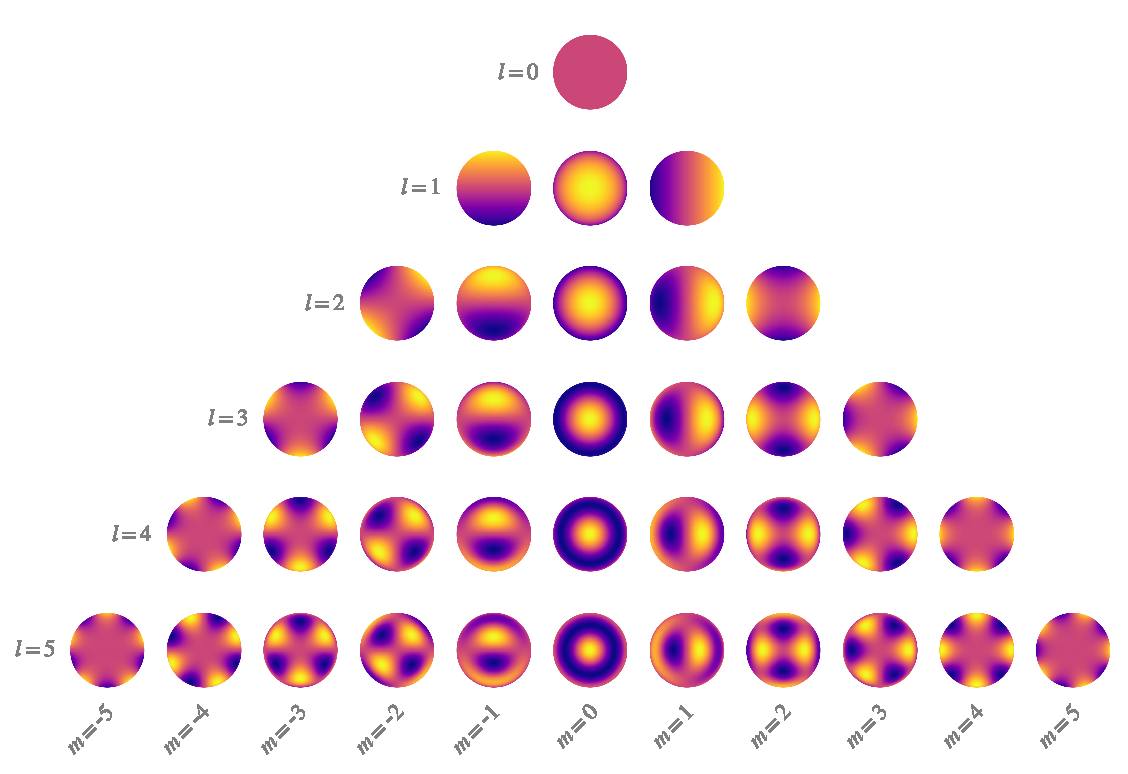
\includegraphics[width=\linewidth]{figures/ylms.pdf}
        \oscaption{ylms}{%
            The real spherical harmonics in the polar frame up to
            $l = 5$. Rows correspond to the degree $l$ and columns to
            the order $m$. The set of all spherical harmonics forms a
            complete, orthogonal basis on the sphere.
            \label{fig:ylms}
        }
    \end{centering}
\end{figure}

Before we dive in, it is useful to introduce the spherical harmonics,
a set of orthogonal functions on the surface of the sphere which we will use
to describe the intensity field on the surface of a star
(Figure~\ref{fig:ylms}). As we will see below,
the spherical harmonics are a particularly convenient basis in which to
describe star spot distributions%
\footnote{There are, of course, drawbacks to using this basis:
    in particular, the spherical harmonics are smooth, continuous functions that
    struggle (at finite degree $l$) to capture high resolution features such as
    small star spots. We discuss this point at length in \S\ref{sec:tinyspots},
    where we show that our model is useful even when applied to stars with spots
    smaller than the effective resolution of the GP.}, as they will allow us to compute
moments of the intensity distribution analytically. And of more immediate concern,
\citet{Luger2019} showed that there is a linear relationship between the
spherical harmonic expansion of a stellar surface and the total disk-integrated
flux $\mathbf{f}$ (i.e., the light curve)
one would observe as the star rotates about a fixed axis.
If the stellar surface intensity is described by the spherical harmonic
coefficient vector $\mathbf{y}$, the flux is given by
%
\begin{align}
    \label{eq:fAy}
    \mathbf{f} = \mathbf{1} + \pmb{\mathcal{A}} \, \mathbf{y}
    \quad,
\end{align}
%
where $\mathbf{1}$ is the ones vector and
$\pmb{\mathcal{A}}$ is the \starry
design matrix, a purely linear operator that transforms from the spherical
harmonic basis to the flux basis; it is implicitly
a function of the stellar inclination $I$, the stellar
rotation period $P$, the stellar limb darkening coefficients, etc.
(see Appendix~\ref{sec:starry} for details).

\subsection{Computing the GP}
\label{sec:gp}
%

Let
$\mathbf{f} = \left( f_0 \, f_1 \, \cdots \,  f_{K-1} \right)^\top$
denote a vector of $K$ flux measurements at times
$\mathbf{t} = \left( t_0 \,  t_1 \,  \cdots \, t_{K-1} \right)^\top$,
defined in units such that a star with no spots on it will have
$\mathbf{f} = \mathbf{1}$.
Conditioned on certain physical properties of the
star
(such as its inclination, rotation period, etc.), $\pmb{\theta}_\star$,
and on certain properties of the  star spots
(such as their sizes, positions, etc.), $\pmb{\theta}_\bullet$,
we wish to compute the mean $\pmb{\mu}(\pmb{\theta}_\star, \pmb{\theta}_\bullet)$ and
covariance $\pmb{\Sigma}(\pmb{\theta}_\star, \pmb{\theta}_\bullet)$
of $\mathbf{f}$. Together, these specify a multidimensional Gaussian
distribution, which we assume fully describes%
\footnote{The \emph{true} distribution of stellar light curves conditioned
    on $\pmb{\theta}_\star$ and $\pmb{\theta}_\bullet$ is not Gaussian, so our
    assumption is formally wrong. But, as the saying goes, \emph{all models are
        wrong; some are useful}. As we will show later, this turns out to be
    an extremely useful assumption.}
how our flux measurements
are distributed:
%
\begin{align}
    \mathbf{f}\left(\pmb{\theta}_\star, \pmb{\theta}_\bullet\right) \sim
    \mathcal{N}\Big(
    \pmb{\mu}\left(\pmb{\theta}_\star, \pmb{\theta}_\bullet\right),
    \,
    \pmb{\Sigma}\left(\pmb{\theta}_\star, \pmb{\theta}_\bullet\right)
    \Big)
\end{align}
%
As with any random variable, the mean and covariance may be computed from
the expectation values of $\mathbf{f}$ and
$\mathbf{f}\,\mathbf{f}^\top$, respectively:
%
\begin{align}
    \label{eq:mean}
    \pmb{\mu}(\pmb{\theta}_\star, \pmb{\theta}_\bullet)
     & = \mathrm{E} \Big[ \mathbf{f} \, \Big| \, \pmb{\theta}_\star, \pmb{\theta}_\bullet \Big]
    \\
    \label{eq:cov}
    \pmb{\Sigma}(\pmb{\theta}_\star, \pmb{\theta}_\bullet)
     & = \mathrm{E} \Big[ \mathbf{f} \, \mathbf{f}^\top \, \Big| \, \pmb{\theta}_\star, \pmb{\theta}_\bullet \Big] - \pmb{\mu}(\pmb{\theta}_\star, \pmb{\theta}_\bullet) \pmb{\mu}^\top(\pmb{\theta}_\star, \pmb{\theta}_\bullet)
    \quad.
\end{align}
%
Given the linear relationship between flux and spherical harmonic
coefficients (Equation~\ref{eq:fAy}),
we may write the mean and covariance of our flux GP as
%
\begin{align}
    \label{eq:mean_f}
    \pmb{\mu}(\pmb{\theta}_\star, \pmb{\theta}_\bullet)
     & = \mathbf{1} + \pmb{\mathcal{A}}(\pmb{\theta}_\star) \, \pmb{\mu}_{\mathbf{y}}(\pmb{\theta}_\bullet)
    \\
    \label{eq:cov_f}
    \pmb{\Sigma}(\pmb{\theta}_\star, \pmb{\theta}_\bullet)
     & = \pmb{\mathcal{A}}(\pmb{\theta}_\star) \, \pmb{\Sigma}_{\mathbf{y}}(\pmb{\theta}_\bullet) \, \pmb{\mathcal{A}}^\top(\pmb{\theta}_\star)
    \quad,
\end{align}
%
where
%
\begin{align}
    \label{eq:mean_y}
    \pmb{\mu}_{\mathbf{y}}(\pmb{\theta}_\bullet)
     & = \mathrm{E} \Big[ \mathbf{y} \, \Big| \, \pmb{\theta}_\bullet \Big]
    \\
    \label{eq:cov_y}
    \pmb{\Sigma}_{\mathbf{y}}(\pmb{\theta}_\bullet)
     & = \mathrm{E} \Big[ \mathbf{y} \, \mathbf{y}^\top \, \Big| \, \pmb{\theta}_\bullet \Big] - \pmb{\mu}_{\mathbf{y}}(\pmb{\theta}_\bullet) \pmb{\mu}_{\mathbf{y}}^\top(\pmb{\theta}_\bullet)
\end{align}
%
are the mean and covariance of the GP in the spherical harmonics basis.
The bulk of the math in this paper (Appendix~\ref{sec:integrals})
is devoted to computing
the expectations in the expressions above, which
are given by the integrals
%
\begin{align}
    \label{eq:exp_y}
    \mathrm{E} \Big[ \mathbf{y} \, \Big| \, \pmb{\theta}_\bullet \Big]
     & =
    \int \mathbf{y}(\mathbf{x} ) \, p(\mathbf{x} \, \big| \, \pmb{\theta}_\bullet)\mathrm{d}\mathbf{x}
    \\
    \label{eq:exp_yy}
    \mathrm{E} \Big[ \mathbf{y} \, \mathbf{y}^\top \, \Big| \, \pmb{\theta}_\bullet \Big]
     & =
    \int \mathbf{y}(\mathbf{x} ) \mathbf{y}^\top(\mathbf{x} ) \, p(\mathbf{x} \, \big| \, \pmb{\theta}_\bullet)\mathrm{d}\mathbf{x}
    \quad,
\end{align}
%
where $\mathbf{x}$ is a random vector-valued variable corresponding to a particular
distribution of features on the surface
and $p(\mathbf{x} \, \big| \, \pmb{\theta}_\bullet)$ is its probability density
function (PDF).
%
In the Appendix we show that for suitable choices of $\pmb{\theta}_\bullet$,
$\mathbf{y}(\mathbf{x})$,
and $p(\mathbf{x} \, \big| \, \pmb{\theta}_\bullet)$, the integrals in the expressions
above have closed form solutions that may be evaluated quickly.
%
In particular, we let the spot hyperparameters of our GP be
%
\begin{align}
    \label{eq:thetaspot}
    \pmb{\theta}_\bullet
     & =
    \left(
    N
    \,\,\,
    c
    \,\,\,
    a
    \,\,\,
    b
    \,\,\,
    r
    \,\,\,
    \Delta
    \right)^\top
    \quad,
\end{align}
%
where $N$ is the number of star spots, $c$ is their contrast,
$a$ and $b$ describe the latitudinal
distribution of the spots, and $r$ and $\Delta$ are the mean and
half-width, respectively, of the distribution of spot radii.
%
The PDF for the radius is a uniform distribution
between $r - \Delta$ and $r + \Delta$ (Appendix \ref{sec:size}),
while
the PDF for the latitude $\phi$ of the spots is a Beta distribution in
$\cos\phi$ with (normalized) shape parameters $a$ and $b$,
which have a one-to-one correspondence to the mean $\mu_\phi$ and
standard deviation $\sigma_\phi$ of the distribution in $\phi$
(Appendix \ref{sec:lat-transform}).
The spot longitude is assumed to be uniformly distributed
(Appendix \ref{sec:lon}). Finally,
the PDFs for the spot contrast and the number of spots are delta functions
centered at $c$ and $N$, respectively (Appendix \ref{sec:contrast}).

In this paper, we assume that the parameters $\pmb{\theta}_\bullet$
described above are the \emph{physically interesting} ones. That is,
given a set of $M$ light curves
$\left( \mathbf{f}_0 \, \mathbf{f}_1 \, \cdots \,  \mathbf{f}_{M-1} \right)^\top$,
we wish to infer the statistical properties of the star spots, encoded in
the entries of the vector $\pmb{\theta}_\bullet$.
%
This is typically a tall order, since it requires marginalizing over all
the nuisance parameters, which include the nitty-gritty details of the
size, contrast, and location of \emph{every spot} on \emph{every star}
in the sample. Fortunately, however, the Gaussian process we constructed
does just that. Specifically, given the mean and covariance of the process,
we are able to directly evaluate the log marginal likelihood of the $m^\mathrm{th}$
dataset
conditioned on a specific value of $\pmb{\theta}_\bullet$ (and $\pmb{\theta}_\star$):
%
\begin{align}
    \label{eq:log-like}
    \resizebox{.9\hsize}{!}{$
        \ln \mathcal{L}_m\left(\pmb{\theta}_\star, \pmb{\theta}_\bullet\right)
        =
        -\frac{1}{2}
        \mathbf{r}_m^\top\left(\pmb{\theta}_\star, \pmb{\theta}_\bullet\right)
        \mathbf{K}_m^{-1}\left(\pmb{\theta}_\star, \pmb{\theta}_\bullet\right)
        \mathbf{r}_m\left(\pmb{\theta}_\star, \pmb{\theta}_\bullet\right)
        -
        \frac{1}{2}
        \ln \Big| \mathbf{K}_m\left(\pmb{\theta}_\star, \pmb{\theta}_\bullet\right) \Big|
        -
        \frac{K_m}{2}
        \ln \left( 2 \pi \right)
        \quad,
    $}
\end{align}
%
where
%
\begin{align}
    \mathbf{r}_m\left(\pmb{\theta}_\star, \pmb{\theta}_\bullet\right)
     & \equiv
    \mathbf{f}_m - \pmb{\mu}\left(\pmb{\theta}_\star, \pmb{\theta}_\bullet\right)
\end{align}
%
is the residual vector,
%
\begin{align}
    \mathbf{K}_m\left(\pmb{\theta}_\star, \pmb{\theta}_\bullet\right)
     & \equiv
    \pmb{\Sigma}\left(\pmb{\theta}_\star, \pmb{\theta}_\bullet\right)
    +
    \mathbf{C}_m
\end{align}
%
is the sum of the GP covariance and the data covariance $\mathbf{C}_m$
(which in most cases is a diagonal matrix whose entries
are the squared uncertainty corresponding to each data point in the light curve),
%
$| \cdots |$ denotes the determinant, and $K_m$ is the number of data points.
In an ensemble analysis, the joint marginal likelihood of all datasets is
simply the product of the individual likelihoods, so in log space we have
%
\begin{align}
    \ln \mathcal{L}\left(\pmb{\theta}_\star, \pmb{\theta}_\bullet\right)
     & =
    \sum_{m} \ln \mathcal{L}_m\left(\pmb{\theta}_\star, \pmb{\theta}_\bullet\right)
    \quad.
\end{align}
%
The marginal likelihood may be interpreted as the probability of the data
given the model. Typically, we are interested in the reverse: the probability
of the \emph{model} given the \emph{data}, i.e., the posterior probability
distribution. In later sections we present a comprehensive suite of
posterior inference exercises demonstrating that our GP model is correctly
calibrated, allowing one to efficiently infer statistical properties of star spots
from light curves with minimal bias.


\subsection{Marginalizing over inclination}
\label{sec:inclination}
%
As we mentioned in the previous section,
the equations for the mean and covariance of the flux GP
(Equations~\ref{eq:mean_f} and \ref{eq:cov_f}, respectively) are conditioned
on specific values of the stellar properties $\pmb{\theta}_\star$ and the
spot properties $\pmb{\theta}_\bullet$. To obtain the posterior distribution
for these parameters, we must typically resort to numerical sampling techniques,
which often scale steeply with the number of parameters. It is therefore generally
desirable to keep the total number of parameters small, especially when
employing the GP in an ensemble setting.
In such a setting, we might have light curves from $N_\star$ stars, all of which
we believe to have similar spot properties (perhaps because they have
similar spectral types and rotation periods, for example).
The total number of parameters in our problem is therefore
%
\begin{align}
    N_\theta = N_\star \, \mathrm{dim}(\pmb{\theta}_\star) + 5
    \quad,
\end{align}
%
since each of the stars will have their own set of stellar properties
$\pmb{\theta}_\star$ but will all share the same 5 spot properties
$\pmb{\theta}_\bullet$ (by assumption).
In a typical problem, the stellar parameters might be
%
\begin{align}
    \pmb{\theta}_\star =
    \left(
    I \,\,\,
    P \,\,\,
    u_1 \,\,\,
    u_2
    \right)^\top
    \quad,
\end{align}
%
i.e., the inclination, the rotational period, and some (usually two) limb
darkening coefficients. Thus, for a reasonably sized ensemble of $N_\star=100$
stars, we would have to sample over $N_\theta = 405$ parameters.
While large, this number is certainly not absurd, especially by modern standards.
However, it does pose
a problem when considering how complex the posterior distribution for the
spot mapping problem can be. In addition to strong nonlinear degeneracies
between some of the parameters (such as the contrast $c$ and the
number of spots $N$), the posterior is often multimodal, especially in the
stellar inclinations. While modern sampling schemes such as Hamiltonian
Monte Carlo and Nested Sampling may in principle be able to deal with these
issues, in practice it can be very difficult to obtain convergence in a
reasonable amount of time.

One workaround is to fix the values of $\pmb{\theta}_\star$. This could be done,
for instance, to the rotational period $P$, which can often be estimated with
fairly good accuracy from a periodogram. The limb darkening coefficients could
be fixed at theoretical values, or perhaps their values could be shared among
all stars (and sampled over), given the similarity assumption above.

The inclination, however, is a different matter. Absent prior information
for a particular star (such as a measurement of its projected rotational
velocity $v\sin i$ or the knowledge that it hosts a transiting planet), it
is simply not possible to reliably estimate the inclination in a
pre-processing step. Any light curve statistic one might argue should scale
with inclination---such as the amplitude of the variability---is invariably
degenerate with the spot parameters $\pmb{\theta}_\bullet$. If one knew
$\pmb{\theta}_\bullet$, then perhaps a decent point estimate of $i$ could
be obtained, but in that case the analysis wouldn't be needed in the first place!
%

Fortunately, there is a better way to reduce the number of parameters in
the problem: we can explicitly marginalize over the stellar inclination.
Let
%
\begin{align}
    \label{eq:thetastarbar}
    \bar{\pmb{\theta}}_\star = \left(
    P \,\,\,
    u_1 \,\,\,
    u_2
    \right)^\top
    \quad,
\end{align}
%
be the vector of all stellar parameters \emph{except}
the inclination, where perhaps $P$ is fixed for each star and the limb darkening coefficients
are shared among all stars, as described above.
Then we can write the first two moments of our flux GP as
%
\begin{align}
    \label{eq:einc}
    \mathrm{E} \Big[ \mathbf{f} \, \Big| \, \bar{\pmb{\theta}}_\star, \pmb{\theta}_\bullet \Big]
     & =
    \mathrm{E} \Big[ \mathbf{1} + \pmb{\mathcal{A}} \, \mathbf{y} \, \Big| \, \bar{\pmb{\theta}}_\star, \pmb{\theta}_\bullet \Big]
    \nonumber \\[0.5em]
     & =
    \mathbf{1} + \mathbf{e}_I
\end{align}
%
where we define the first moment integral
%
\begin{align}
    \label{eq:eI}
    \mathbf{e}_I
     & \equiv
    \mathrm{E} \Big[ \pmb{\mathcal{A}} \, \mathbf{y} \, \Big| \, \bar{\pmb{\theta}}_\star, \pmb{\theta}_\bullet \Big]
    \nonumber \\[0.5em]
     & =
    \int
    \pmb{\mathcal{A}}(I, \bar{\pmb{\theta}}_\star) \,
    \mathrm{E} \Big[ \mathbf{y} \, \Big| \, \pmb{\theta}_\bullet \Big]
    p(I) \, \mathrm{d}I
\end{align}
%
and
%
\begin{align}
    \label{eq:Einc}
    \mathrm{E} \Big[ \mathbf{f} \, \mathbf{f}^\top \, \Big| \, \bar{\pmb{\theta}}_\star, \pmb{\theta}_\bullet \Big]
     & =
    \mathrm{E} \Big[ \left(\mathbf{1} + \pmb{\mathcal{A}} \, \mathbf{y}\right) \left(\mathbf{1} + \pmb{\mathcal{A}} \, \mathbf{y}\right)^\top  \, \Big| \, \bar{\pmb{\theta}}_\star, \pmb{\theta}_\bullet \Big]
    \nonumber \\[0.5em]
     & =
    \mathbf{1} \, \mathbf{1}^\top +
    \mathbf{1} \, \mathbf{e}_I^\top +
    \mathbf{e}_I \, \mathbf{1}^\top +
    \mathbf{E}_I
\end{align}
%
where we define the second moment integral
%
\begin{align}
    \label{eq:EI}
    \mathbf{E}_I
     & \equiv
    \int
    \pmb{\mathcal{A}}(I, \bar{\pmb{\theta}}_\star) \,
    \mathrm{E} \Big[ \mathbf{y} \, \mathbf{y}^\top \, \Big| \, \pmb{\theta}_\bullet \Big] \,
    \pmb{\mathcal{A}}^\top(I, \bar{\pmb{\theta}}_\star)
    p(I) \, \mathrm{d}I
    \quad.
\end{align}
%
The expectations inside the integrals in the expressions for
$\mathbf{e}_I$ and $\mathbf{E}_I$
are given by
Equations~(\ref{eq:exp_y_sep}) and (\ref{eq:exp_yy_sep}), respectively.
%
If we are able to perform the integrals in those expressions,
we can \emph{dramatically} reduce the number of
parameters in our ensemble problem.
%
As we show in Appendix~\ref{sec:inclination}, if we assume that stellar
inclinations are distributed isotropically, these integrals
do in fact have closed-form solutions.
%
We may then replace our expressions for the GP mean and covariance with
%
\begin{align}
    \label{eq:mu_marg}
    \pmb{\mu}(\bar{\pmb{\theta}}_\star, \pmb{\theta}_\bullet)
     & = \mathrm{E} \Big[ \mathbf{f} \, \Big| \, \bar{\pmb{\theta}}_\star, \pmb{\theta}_\bullet \Big]
    \nonumber                                                                                                                                                                                                                                       \\
     & = \mathbf{1} + \mathbf{e}_I
    \nonumber                                                                                                                                                                                                                                       \\
     & = \mu \, \mathbf{1}
    \\[0.5em]
    \label{eq:cov_marg}
    \pmb{\Sigma}(\bar{\pmb{\theta}}_\star, \pmb{\theta}_\bullet)
     & = \mathrm{E} \Big[ \mathbf{f} \, \mathbf{f}^\top \, \Big| \, \bar{\pmb{\theta}}_\star, \pmb{\theta}_\bullet \Big] - \pmb{\mu}(\bar{\pmb{\theta}}_\star, \pmb{\theta}_\bullet) \pmb{\mu}^\top(\bar{\pmb{\theta}}_\star, \pmb{\theta}_\bullet)
    \nonumber
    \\
     & =
    \mathbf{E}_I
    -
    \mathbf{e}_I \,
    \mathbf{e}_I^\top
\end{align}
%
and use these to compute the marginal likelihood instead. Note that in the
expression for the mean we made explicit use of the fact that the longitudinal
isotropy of the process results in $\mathbf{e}_I = e_I \, \mathbf{1}$ being
constant (see Appendix~\ref{sec:inc-mom1}), so the process mean is likewise
constant, with $\mu = 1 + e_I$.

\subsection{The baseline problem}
\label{sec:baseline}

There is one final subtle---but extremely important---point that remains to
be discussed in our derivation of a Gaussian process for stellar
rotation. Thus far we have cast the light curve problem in a typical GP inference
setting: we model our observations $\mathbf{f}$ as
a multidimensional random variable distributed as a multivariate Gaussian with mean vector
$\pmb{\mu}$ and covariance matrix $\pmb{\Sigma}$. However, in the context of
relative photometry, the mean $\pmb{\mu}$ is typically \emph{unobservable}.
%
To understand why, consider what
$\pmb{\mu}(\pmb{\theta}_\star, \pmb{\theta}_\bullet)$ actually represents:
it is the expected value
of the flux
for a star with certain properties $\pmb{\theta}_\star$ and $\pmb{\theta}_\bullet$,
\emph{in units of the flux one would measure if the star had no spots}.
We do not observe in these units: rather, we observe in units of counts on
the detector, which depend on the luminosity of the star, the distance to
the star, and various properties of the telescope. Even if we knew all these
things, we would still need to know the intrinsic photospheric brightness
in order to properly normalize our dataset for direct application of
the Gaussian process.

Instead, what astronomers typically do is to self-normalize their data:
i.e., divide the flux by the mean, median, maximum, or some similar
statistic of the light curve. This operation folds the unknowability of
the flux baseline under the rug and transforms the light curve into a \emph{relative}
measurement of the star's temporal variability. While relative measurements
are typically what we are interested in anyways, this normalization procedure
has two significant drawbacks: (1) it introduces a new set of perfect degeneracies
in the modeling and (2) it can substantially change the covariance structure
of the dataset.

The first point is illustrated in the toy example in
Figure~\ref{fig:mean_normalization}. As it has been pointed out before \xxx{(?)},
we will not spend too much time discussing it, other than to say that the
flux normalization introduces a degeneracy between the total spot coverage
of a star and the contrast of any individual feature on the surface.
While this is a formally perfect degeneracy for a single light curve, we can
again resort to ensemble statistics across many light curves to break it;
we discuss this further in \S\ref{sec:breaking_baseline_degeneracy}.

\begin{figure}[ht!]
    \begin{centering}
        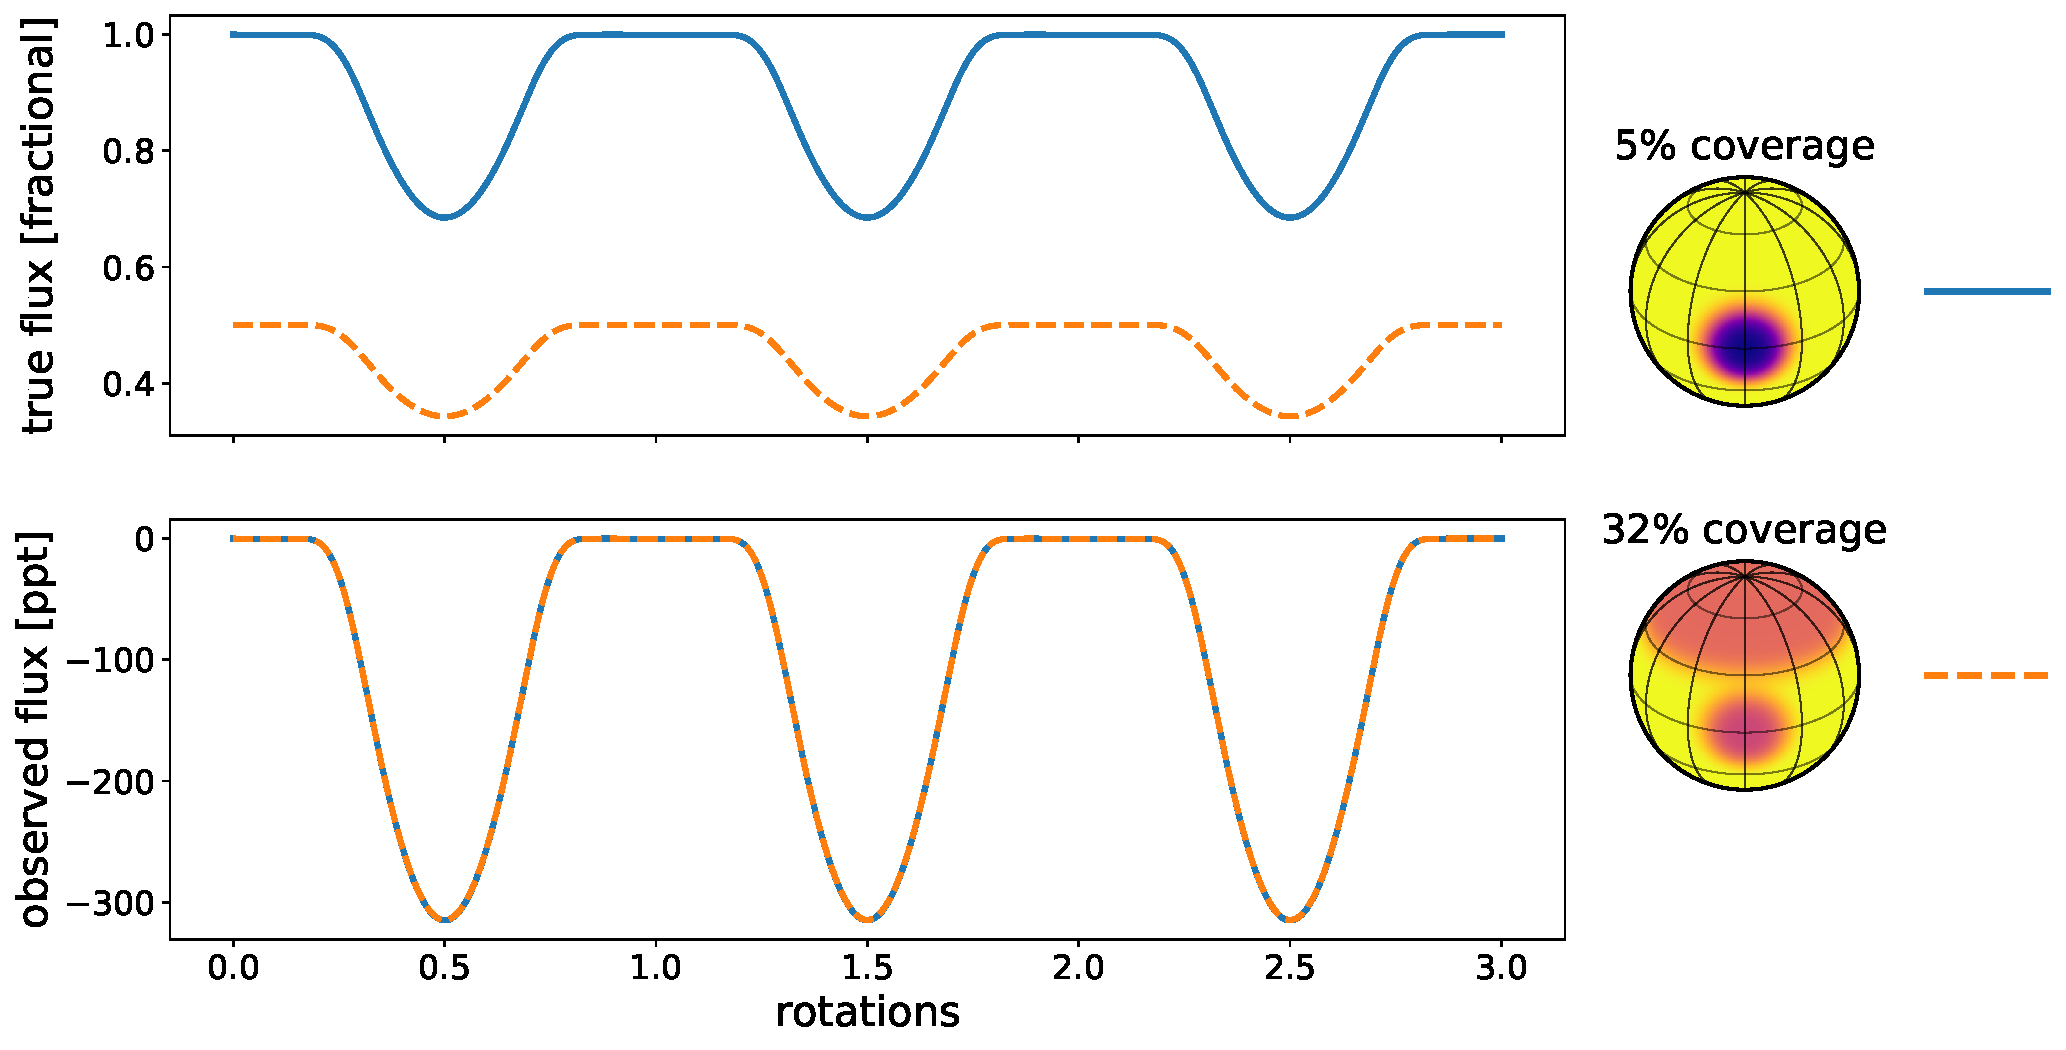
\includegraphics[width=\linewidth]{figures/mean_normalization.pdf}
        \oscaption{mean_normalization}{%
            An example of the baseline problem.
            \emph{Top:} Consider a star with a single
            equatorial spot of contrast $c$ viewed at a certain inclination.
            The total flux (in some units) as a function of time is shown as
            the blue curve. Now, consider a second star,
            identical in all respects to the first, except that (1) the equatorial spot
            has half the contrast (i.e., $\nicefrac{c}{2}$); and (2) there is
            a second, large spot centered on the pole. The corresponding light
            curve is shown as the dashed orange curve.
            The orange light curve is different from the blue one in two ways:
            (1) since the equatorial spot has half the contrast, the amplitude of the associated
            dips in the light curve is half that of the first star; and
            (2) since the polar spot is azimuthally symmetric, its only
            contribution is a net darkening at all phases.
            \emph{Bottom:} The true baseline level of a stellar
            light curve, which corresponds to the flux one would measure in the
            absence of any spots, is almost always unknown. Photometric measurements
            are therefore meaningful only in a relative sense, i.e., as deviations from
            the mean, median, or maximum level of the light curve.
            The bottom panel shows the same two light curves, this time plotted as
            deviations in parts per thousand (ppt) from their respective maxima.
            To the observer, the two light curves are \emph{indistinguishable}.
            In the absence of baseline information, there
            exists a perfect degeneracy between the total spot coverage
            and the contrast of any individual feature on the surface.
            \label{fig:mean_normalization}
        }
    \end{centering}
\end{figure}

The second point is of more immediate concern, since we must correct our
expression for the covariance matrix
$\pmb{\Sigma}(\pmb{\theta}_\star, \pmb{\theta}_\bullet)$ if we are to
use our GP to model normalized light curves. For definiteness, let us
consider only mean-normalized light curves.%
\footnote{In practice, the expressions derived below also work well
    for median-normalized light curves, since the distribution of the GP sample median
    is usually close to the distribution of sample mean.}%
Since we are dividing the
flux by the mean, one might imagine that we could simply divide the
covariance matrix by the square of the mean and call it a day. However,
this is incorrect, since we must be careful to distinguish between the
\emph{sample} mean and the \emph{process} mean. When normalizing a light
curve by the mean, the operation we perform is
%
\begin{align}
    \label{eq:ftilde}
    \tilde{\mathbf{f}\hspace{0.2em}} & = \frac{\mathbf{f}}{\left<f\right>}
    \quad,
\end{align}
%
where $\tilde{\mathbf{f}\hspace{0.2em}}$ is the normalized, unit-mean light curve,
$\mathbf{f}$ is the measured light curve (in detector counts), and
$\left<f\right>$ is the \emph{sample} mean: i.e., the average value of
a given star's light curve (which we model as a sample from our GP).
This may be close to but is in general different from the \emph{process} mean,
$\pmb{\mu}(\pmb{\theta}_\star, \pmb{\theta}_\bullet)$, since the mean of
a draw from the GP is itself normally distributed with a variance that scales
with the GP variance.

Computing the covariance of the normalized process is tricky, especially
because the normalized process is \emph{not} strictly Gaussian: the distribution
has heavy tails due to the fact that $\tilde{\mathbf{f}\hspace{0.2em}}$ diverges as
the sample mean approaches zero. In fact, because of these tails, the covariance
of the normalized process is formally \emph{infinite}, since the probability of
drawing a sample whose mean is arbitrarily close to zero is finite.

If this is all starting to sound like a bad idea, that's because it is!
A much safer approach is to resist the temptation to normalize the light curve
and instead model the unknown baseline as a latent variable. However,
this would require an extra parameter \emph{for every light curve}, so the
computational savings we achieved by marginalizing out the inclination
would be gone. Fortunately, in practice, the variance of a stellar light curve
is usually small compared to its mean: stellar variability amplitudes are
typically at the level of a few percent or lower. When this is the case,
the probability of drawing a GP sample whose mean is close to zero is
extremely small, and we can make use of the approximate expression derived
in \citet{Luger2020} for the covariance of a normalized Gaussian process:
%
\begin{align}
    \label{eq:SigmaTilde}
    \tilde{\pmb{\Sigma}}
     & \approx
    \frac{A}{\mu^2} \pmb{\Sigma} +
    z \Big(
    (A + B) \, (\mathbf{1} - \mathbf{q}) \, (\mathbf{1} - \mathbf{q})^\top
    - A \, \mathbf{q} \, \mathbf{q}^\top
    \Big)
    \quad,
\end{align}
%
where
%
\begin{align}
    z & \equiv \frac{\left< \Sigma \right>}{\mu^2}
\end{align}
%
is the ratio of the average element in $\pmb{\Sigma}$
to the square of the mean of the Gaussian process,
$\mathbf{q}$ is the ratio of the average of each row in $\pmb{\Sigma}$
to the average element in $\pmb{\Sigma}$, and $A$, $B$ are
order unity and zero scalars, respectively,
given by the optimally-truncated diverging series
%
\begin{align}
    \label{eq:baseline_alpha}
    A
     & \equiv
    \sum\limits_{n=0}^N
    \frac{(2n + 1)!}{2^n \, n!}
    z^n
    \\[1em]
    \label{eq:baseline_beta}
    B
     & \equiv
    \sum\limits_{n=0}^N
    \frac{2n(2n + 1)!}{2^n \, n!}
    z^n
    \quad,
\end{align}
%
where $N$ is the largest value for which the series coefficient at $N$ is
smaller than the coefficient at $N - 1$. In the expressions above, it is
assumed that the mean $\pmb{\mu}$ is constant, i.e., $\pmb{\mu} = \mu\, \mathbf{1}$.
Since our Gaussian process is azimuthally isotropic (i.e., no preferred
longitude), that is the case throughout this paper.

What Equation~(\ref{eq:SigmaTilde}) allows us to do is effectively marginalize over
the unknown baseline by modeling the \emph{normalized} flux as a draw
from a Gaussian process:
%
\begin{align}
    \tilde{\mathbf{f}\hspace{0.2em}}
    \left(\pmb{\theta}_\star, \pmb{\theta}_\bullet\right)
    \sim
    \mathcal{N}\left(
    \mathbf{1},
    \tilde{\pmb{\Sigma}} \left(\pmb{\theta}_\star, \pmb{\theta}_\bullet\right)
    \right)
    \quad.
\end{align}
%
This is appropriate as long as the quantity $z \ll 1$, for which the true
distribution of $\tilde{\mathbf{f}\hspace{0.2em}}$ is approximately Gaussian. In practice,
we recommend employing this trick only for $z \lesssim 0.02$, for which the
error in the approximation to the covariance is less than $10^{-6}$.
In cases where the light curve variability exceeds a few percent, we recommend
modeling the baseline in each light curve as a latent variable, as discussed
above.

\begin{figure}[ht!]
    \begin{centering}
        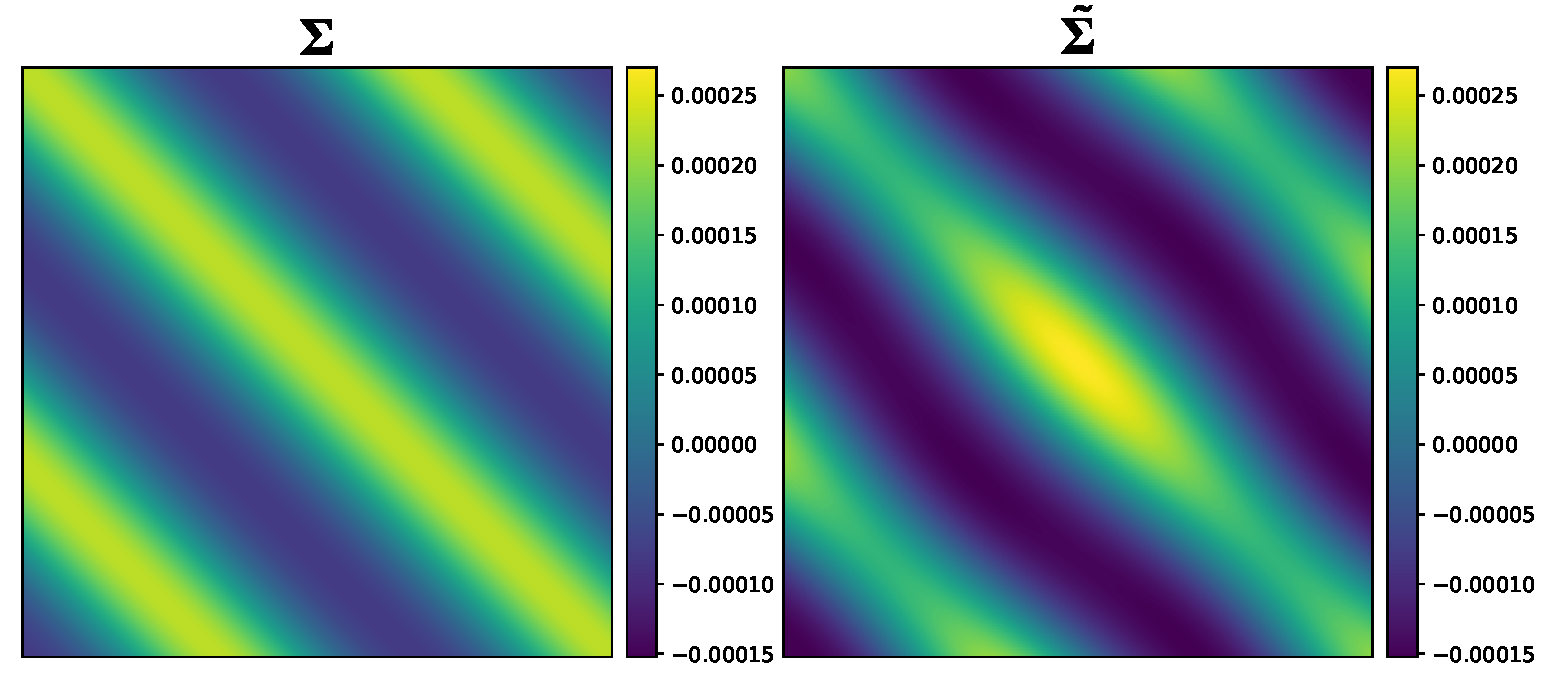
\includegraphics[width=\linewidth]{figures/normgp.pdf}
        \oscaption{normgp}{%
            An example of a flux covariance matrix $\pmb{\Sigma}$ for a
            \starry process (left) and the corresponding covariance of the
            normalized process (right), computed from Equation~(\ref{eq:SigmaTilde}).
            In addition to an offset and an overall scaling relative to the
            original covariance matrix, the covariance of the normalized process
            is discernibly non-stationary.
            \label{fig:normgp}
        }
    \end{centering}
\end{figure}

Figure~\ref{fig:normgp} shows an example of a covariance matrix normalized
according to the procedure outlined above. The principal difference between
the normalized covariance and the original covariance is an overall
scaling and a small offset. However, the normalization also results in
the process becoming non-stationary: the covariance between two points in
a light curve is now slightly dependent on their phases.

\subsection{Summary}
\label{sec:summary}
%
As the computation of the GP relies on many interdependent equations
scattered throughout the previous sections and the Appendix, it
is useful to summarize the procedure for the case where we marginalize
over the inclination (\S\ref{sec:inclination}) and the light curves are
normalized to their means (\S\ref{sec:baseline}), which is likely to be the primary
use case for our algorithm.

We model the mean-normalized flux $\tilde{\mathbf{f}\hspace{0.2em}}$
(Equation~\ref{eq:ftilde}) as a Gaussian process:
%
\begin{align}
    \tilde{\mathbf{f}\hspace{0.2em}}
    \left(\bar{\pmb{\theta}}_\star, \pmb{\theta}_\bullet\right)
    \sim
    \mathcal{N}\left(
    \mathbf{1},
    \tilde{\pmb{\Sigma}} \left(\bar{\pmb{\theta}}_\star, \pmb{\theta}_\bullet\right)
    \right)
    \quad,
\end{align}
%
where $\bar{\pmb{\theta}}_\star$ are hyperparameters describing the star, such
as the rotation period and limb darkening coefficients
(Equation~\ref{eq:thetastarbar}),
$\pmb{\theta}_\bullet$ are the hyperparameters describing the star spot
distribution, including the number of spots, their contrast, parameters
describing their latitudinal distribution, and parameters describing their
radius distribution (Equation~\ref{eq:thetaspot}),
and $\tilde{\pmb{\Sigma}}$ is the covariance of the normalized process
(Equation~\ref{eq:SigmaTilde}). This covariance is a straightforward correction to the
true covariance of the process, which accounts for
changes of scale and phase dependence introduced by the common process of
normalizing light curves to a mean of unity. It depends on the
true (constant) mean $\mu$
and true covariance $\pmb{\Sigma}$,
given by Equations~(\ref{eq:mu_marg}) and (\ref{eq:cov_marg}),
respectively.
Those expressions in turn depend on the inclination expectation integrals
$e_I$ (Appendix~\ref{sec:inc-mom1}) and $\mathbf{E}_I$
(Appendix~\ref{sec:inc-mom2}). Those, in turn, depend on the first and
second moments of the distribution of spherical harmonic coefficient vectors,
$\mathrm{E}\left[ \mathbf{y} \big| \pmb{\theta}_\bullet \right]$
and
$\mathrm{E}\left[ \mathbf{y} \, \mathbf{y}^\top \big| \pmb{\theta}_\bullet \right]$,
given by Equations~(\ref{eq:exp_y_sep}) and (\ref{eq:exp_yy_sep}), respectively.
To compute those, we must evaluate four nested integrals
(Equations~\ref{eq:e1}--\ref{eq:e4} for the first moment
and \ref{eq:E1}--\ref{eq:E4} for the second moment), corresponding to integrals
over the radius, latitude, longitude, and contrast distributions, respectively.
The computation of these integrals is discussed at length in Appendix~\ref{sec:integrals}.

While lengthy (and quite tedious), all of the computations described above rely
on equations whose solutions have a closed form.%
%
\footnote{The exception to this is the
    normalization correction (\S\ref{sec:baseline}), which depends on a rapidly
    converging series and thus adds negligible overhead to the computation.}
%
Moreover, most of the terms in the expectation vectors and matrices may
be computed recursively, and many may be pre-computed, as they do not
depend on user inputs.
%
It is therefore possible to evaluate $\tilde{\pmb{\Sigma}}$ in an extremely
efficient manner. In \S\ref{sec:implementation} we discuss our
implementation of the algorithm in a user-friendly \Python package.


\section{Discussion}
\label{sec:discussion}

\subsection{Ensemble Analyses}
\label{sec:ensemble}

Figure~\ref{fig:nullspace_ensemble} shows the posterior shrinkage
as a function of spherical harmonic degree for three different
(purely hypothetical) scenarios: a single high signal-to-noise ratio (SNR)
observation of a stellar light curve at a random
observer inclination (thin blue curves), a set of three observations
of the same star at three \emph{different} random inclinations (thin
orange curves), and a set of ten observations at ten different
random inclinations (thin green curves).
The denser, opaque curves show the average for each scenario over 300 trials.
The posterior shrinkage $R$ for a given
spherical harmonic coefficient is computed from
%
\begin{align}
    R \equiv 1 - \lim\limits_{\sigma_0^2 \rightarrow \infty}
    \frac{\sigma^2}{\sigma_0^2}
\end{align}
%
where $\sigma_0^2$ is the prior variance
and $\sigma^2$ is the posterior variance.
It is a measure of how informative a measurement is about a
given mode on the surface in the limit of infinite SNR
and is independent of what the stellar surface actually looks like.
If, at infinite SNR and with a completely uninformative prior,
a particular mode can be learned exactly from a dataset, the posterior
shrinkage is defined to be unity. Conversely, if the data is completely
unconstraining, $R$ will tend to zero.

\begin{figure}[ht!]
    \begin{centering}
        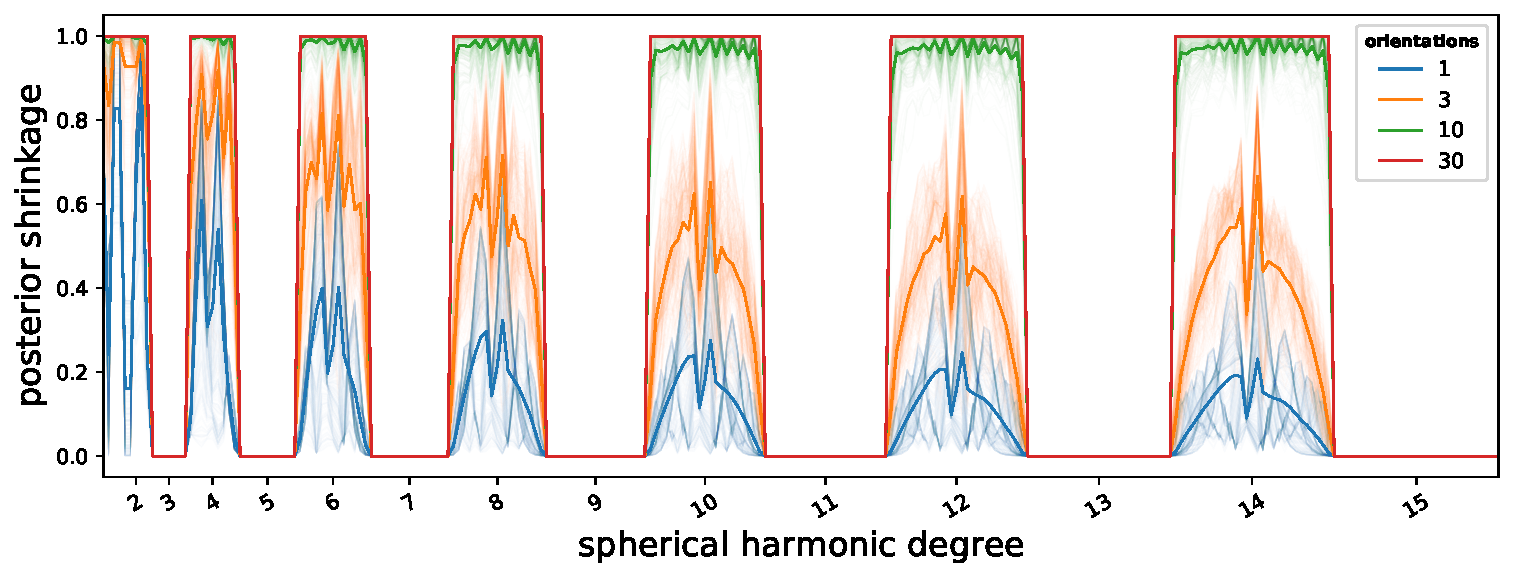
\includegraphics[width=\linewidth]{figures/nullspace_ensemble.pdf}
        \oscaption{nullspace_ensemble}{%
            Posterior shrinkage as a function of spherical harmonic degree
            for a hypothetical scenario in which an observer can measure a
            stellar light curve at a single random inclination (thin blue curves),
            at 3 random inclinations (thin orange curves), and at 10 random
            inclinations (thin green curves). The thicker curves correspond to
            the mean shrinkage for each experiment.
            The information content in the light curve of a star observed
            from a single vantage point approaches zero as $l$
            increases. However, observing the star from many vantage points
            allows one to recover nearly all of the information in the
            even spherical harmonic modes.
            While this thought experiment is not possible in practice for
            a single star, it is extremely relevant to ensemble analyses of statistically
            similar stars.
            \label{fig:nullspace_ensemble}
        }
    \end{centering}
\end{figure}

Let us first consider the blue curves, in which a light curve is
collected from a star viewed at a single random inclination (which, of course, is
all we can do from our fixed vantage point on Earth).
For some of the low-degree modes, the shrinkage is relatively high: it is
fairly easy to constrain the dipole moment from a light curve, as this is
usually the dominant sinusoidal signal. However, as the degree $l$
increases, the shrinkage decreases dramatically: at $l = 14$, corresponding
to features on scales of roughly $15^\circ$, the light curve
can only tell us about $\sim 10\%$ of the total information about what the
surface looks like. As $l$ increases further, $R$ tends to zero.
Another important feature of the shrinkage is that it is exactly zero for
all odd-degree modes above $l = 1$. This is a well-known fact: all odd spherical
harmonics other than the dipole are in the null space \emph{regardless of
    inclination} \citep[e.g.,][]{Luger2019}. In other words, these spherical
harmonics are perfectly antisymmetric in projection over the unit disk
when viewed from any orientation. Absent structure to break these symmetries
(see \S\ref{sec:limbdark}), we simply cannot learn anything about these modes from
stellar light curves. If we average over the shrinkage for all modes up to $l=15$,
we find that a single light curve measurement can only tell us $\sim 9\%$
of the information about the surface.

The orange curves correspond to the scenario in which we can collect light curves
from a star viewed at three different random inclinations. This is obviously
impossible in practice, but it is still instructive as a thought experiment.
Interestingly, the shrinkage increased at all even spherical harmonic degrees
(the odd degrees, as we mentioned above, are always invisible).
Note that since we are in the limit of infinite SNR, the fact that we have
three times the data as we did in the previous scenario is irrelevant: the
increase in the shrinkage is instead due to the fact that our observations
from different vantage points broke some degeneracies in the problem.
This is a consequence of the fact that the null space (for the even modes)
is a strong function of the inclination: modes that are invisbile
at one inclination can actually project into the flux at a different inclination.
If we average over all modes, we obtain a total shrinkage of $\sim 24\%$
for $l\leq15$ in this case.

Finally, the green curves correspond to observations taken at ten random
inclinations. In this scenario, the posterior shrinkage is nearly $100\%$
for all even modes (it asymptotically approaches $100\%$ as the number
of light curves increases further). The total shrinkage is $\sim 47\%$
and approaches $50\%$ as both $l_\mathrm{max}$  and the number of light curves
tend to infinity. Thus, if we were able to measure a light curve of a star
from many different inclinations, the null space would consist \emph{only}
of the odd modes, and our data would tell us exactly half of all the
information about the surface.

As we mentioned above, it is obviously not possible to observe a \emph{single}
star from many different inclinations (at least not at present!).
However, it is certainly the case that we can observe \emph{many} stars
at a wide range of inclinations. Those stars certainly have different
surface intensity distributions, but what if we restricted ourselves to
light curves of ``similar'' stars?

\subsection{Caveats}
\label{sec:caveats}
The true process is not Gaussian. See Figure~\ref{fig:nongaussianity}.
\begin{figure}[ht!]
    \begin{centering}
        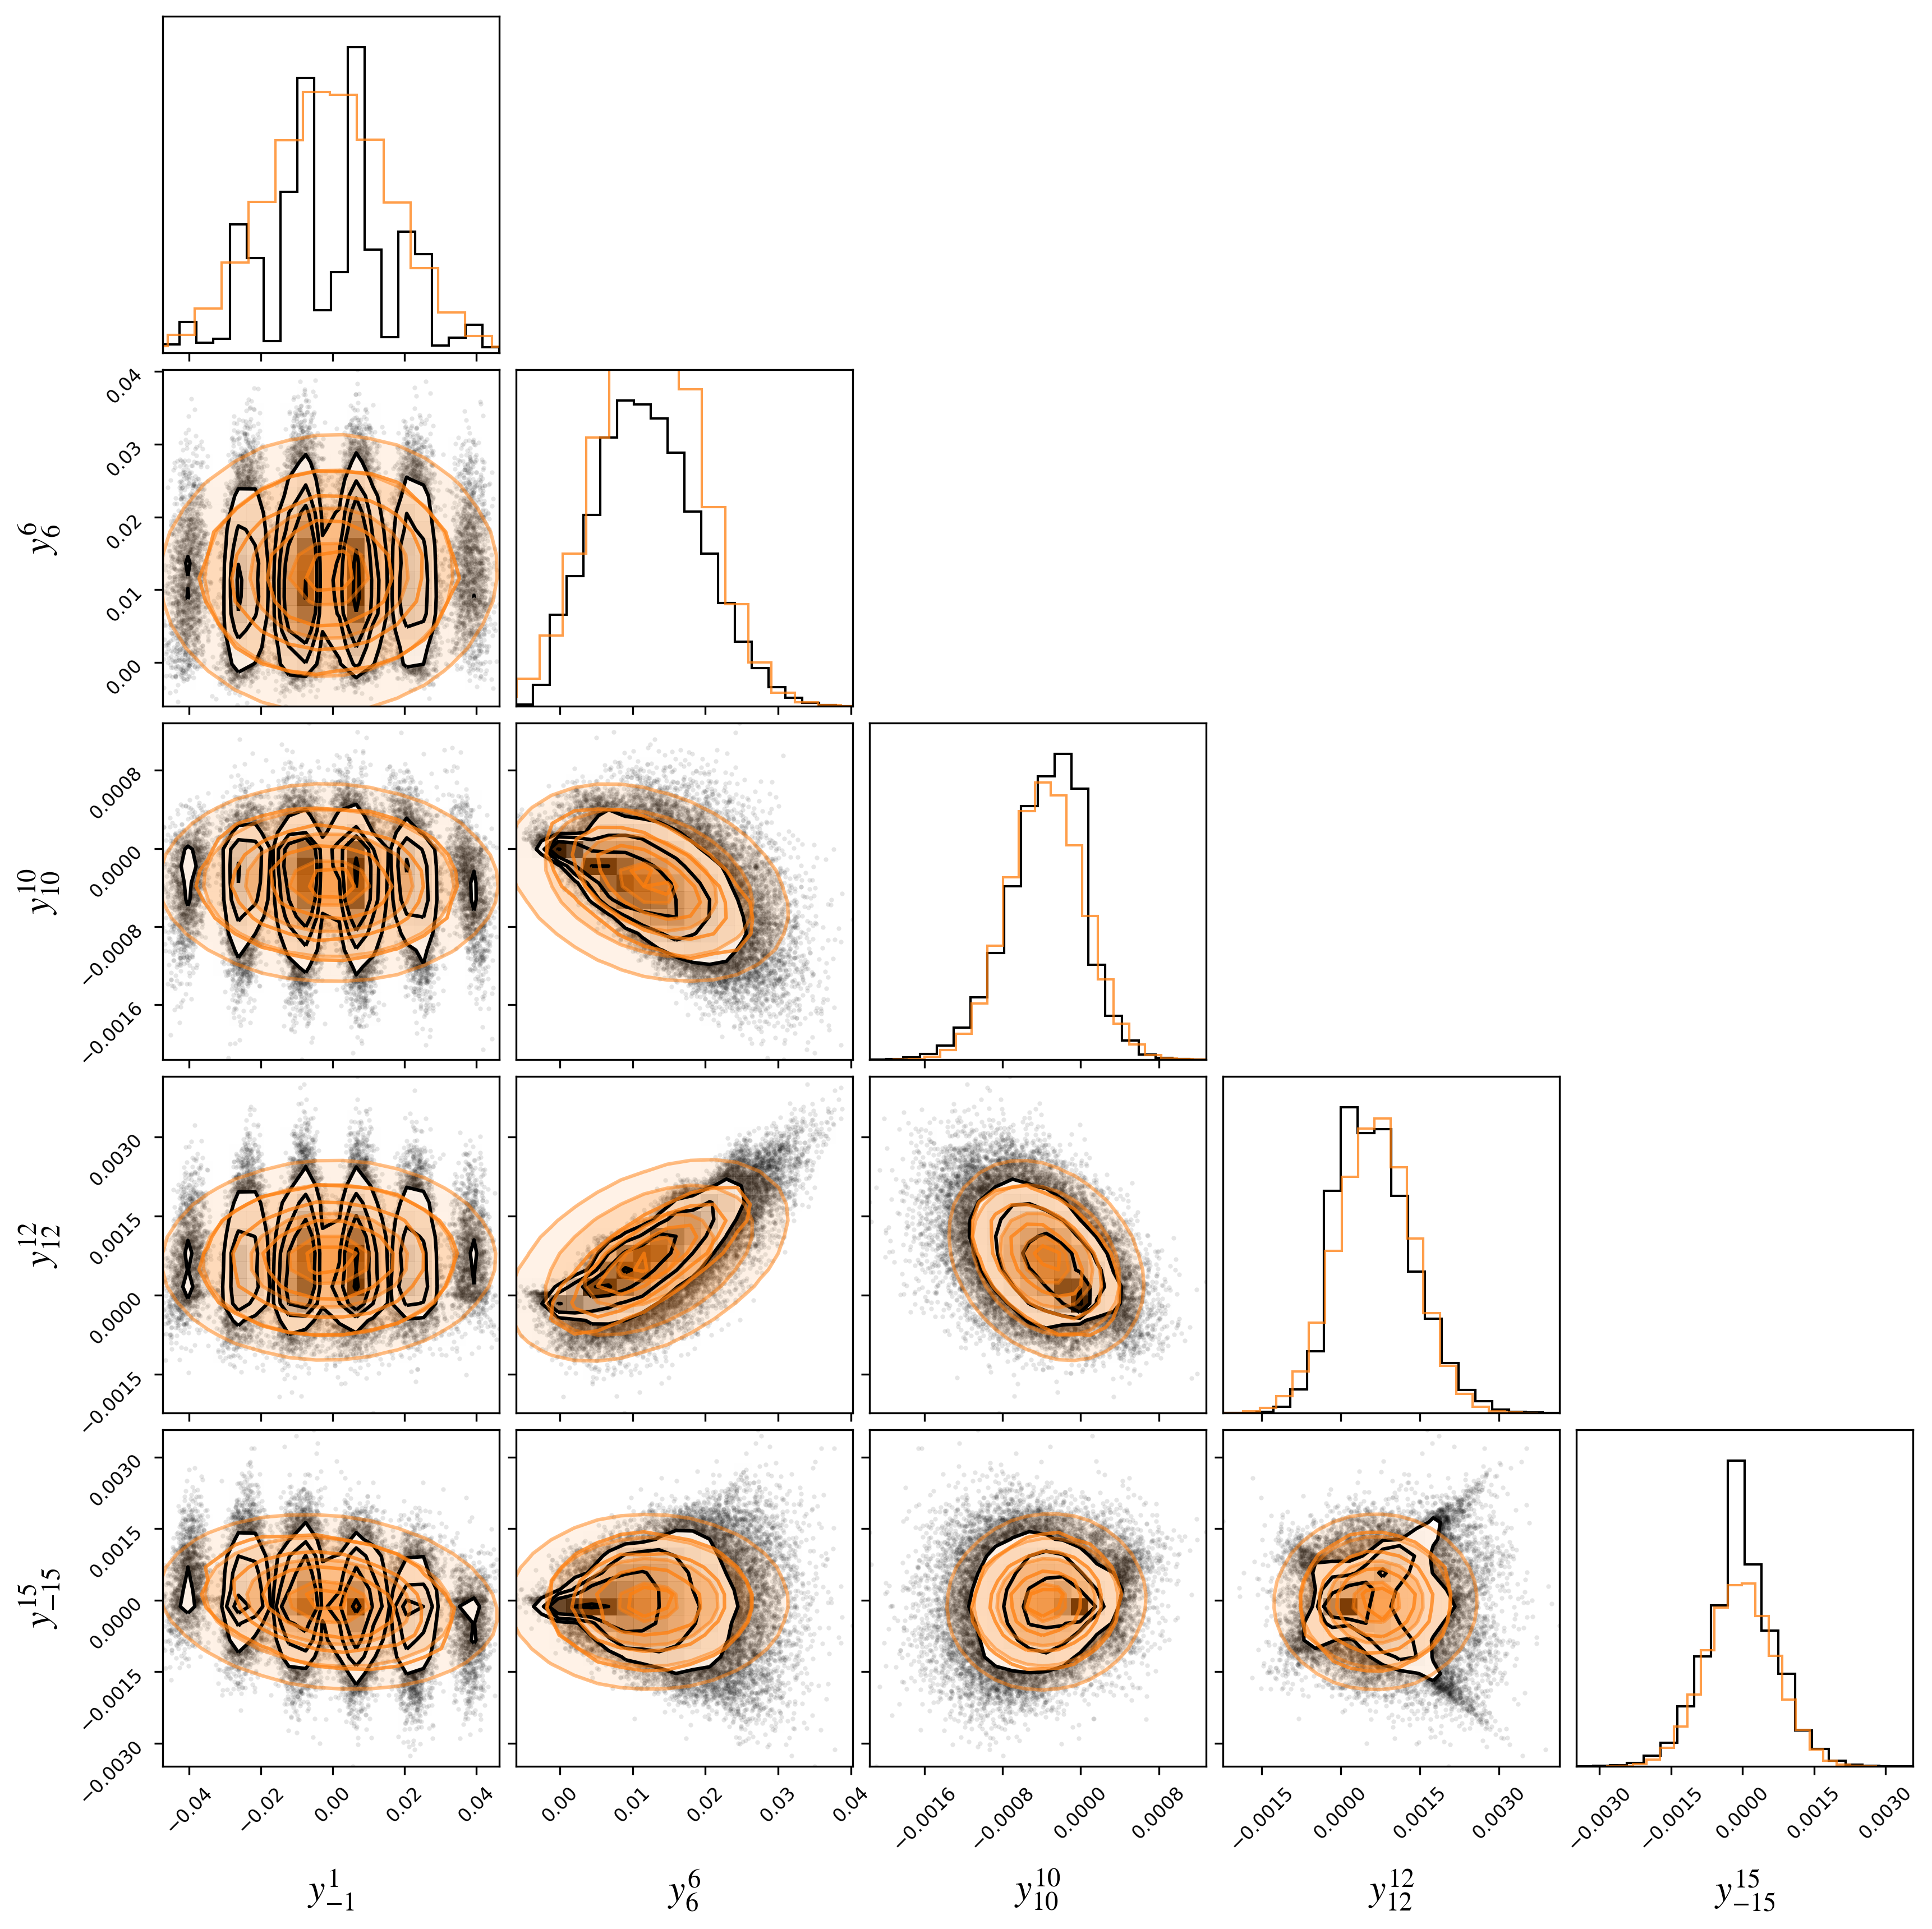
\includegraphics[width=\linewidth]{figures/nongaussianity.pdf}
        \oscaption{nongaussianity}{%
            Corner plot showing the joint distributions of select spherical
            harmonic coefficients corresponding to the $l=15$ expansion of
            $5\times 10^{4}$ stellar surface maps drawn from a certain
            star spot distribution (black points and contours).
            At $l=15$ there are 256 coefficients in total;
            we chose five of the coefficients with the most odd-looking
            distributions to illustrate the non-Gaussianity of the process.
            In addition to non-linear correlations, skewness, and the
            existence of points of very high curvature, some of the distributions
            are also multi-modal.
            The orange contours show slices of the Gaussian approximation to
            the joint distribution; this is the approximation adopted in
            this paper.
            \label{fig:nongaussianity}
        }
    \end{centering}
\end{figure}

%
%
%
%

\appendix

%
%
%
%

\section{Notation}
\label{sec:notation}
%
Unless otherwise noted, we adopt
the following conventions throughout this paper:
integers are represented by italic uppercase letters (i.e., $N$),
scalars are represented by italic lowercase
letters (i.e., $x$), column vectors are
represented by boldface lowercase letters
($\mathbf{x}$), and matrices are represented
by boldface capital letters ($\mathbf{X}$). In general, the elements of a vector
$\mathbf{x}$ are denoted $x_i$ and the elements of a matrix $\mathbf{X}$
are denoted $X_{i,j}$. Importantly, we make a distinction between
quantities like $X_{i,j}$ and $\mathbf{X}_{i,j}$: the former is a scalar
element of a matrix, while the latter is a \emph{matrix}, which is itself
a component of a higher-dimensional (in this case, 4-dimensional) linear
operator. Thus, lowercase bold symbols \emph{always} represent vectors, and
uppercase bold symbols \emph{always} represent matrices.

The exception to our indexing notation is if the vector or matrix
represents a quantity in the spherical harmonic basis, in which case we use
\emph{two} indices to represent a scalar vector element, $x^l_m$, and \emph{four}
indices to represent a scalar matrix element, $X^{l,l'}_{m,m'}$.
%
The upper indices corresponds to the spherical harmonic degree,
$l \in [0, l_{\mathrm{max}}]$ and $l' \in [0, l_{\mathrm{max}}]$,
while the lower indices correspond to the
spherical harmonic order, $m \in [-l, l]$ and $m' \in [-l', l']$.
%
Vector elements are arranged in order of increasing $l$ and,
within each $l$, in order of increasing $m$.
For example, a vector $\mathbf{x}$
representing a quantity in the spherical harmonic basis up to degree
$l_\mathrm{max}$ has components given by
%
\begin{align}
    \mathbf{x}
     & =
    \left(
    x^0_0 \,\,\,
    \,\,\,\,\,\,
    x^1_{-1} \,\,\,
    x^1_{0} \,\,\,
    x^1_{1} \,\,\,
    \,\,\,\,\,\,
    \cdots \,\,\,
    \,\,\,\,\,\,
    x^{l_\mathrm{max}}_{-l_\mathrm{max}}
    \cdots \,\,
    x^{l_\mathrm{max}}_{l_\mathrm{max}} \,\,\,
    \right)^\top
    \quad,
\end{align}
%
while a matrix $\mathbf{X}$ in the same basis has components given by
%
\begin{align}
    \setstackgap{L}{1.25\baselineskip}
    \fixTABwidth{T}
    \mathbf{X} =
    \parenMatrixstack{
    X^{0,0}_{0,0}  &  & X^{0,1}_{0,-1}  & X^{0,1}_{0,0}  & X^{0,1}_{0,1}  &        \\
                   &  &                 &                &                &        \\
    X^{1,0}_{-1,0} &  & X^{1,1}_{-1,-1} & X^{1,1}_{-1,0} & X^{1,1}_{-1,1} &        \\
    X^{1,0}_{0,0}  &  & X^{1,1}_{0,-1}  & X^{1,1}_{0,0}  & X^{1,1}_{0,1}  &        \\
    X^{1,0}_{1,0}  &  & X^{1,1}_{1,-1}  & X^{1,1}_{1,0}  & X^{1,1}_{1,1}  &        \\
                   &  &                 &                &                & \ddots
    }\quad.
\end{align}
%
For completeness, the element of a spherical harmonic vector $\mathbf{x}$ with
degree $l$ and order $m$ is at (flattened) index
%
\begin{align}
    \label{eq:n}
    n = l^2 + l + m
    \quad.
\end{align}
%
Conversely, the element at (flattened) index $n$ has degree and order
%
\begin{align}
    \label{eq:lm}
    \begin{split}
        l & = \floor{\sqrt{n}}
        \\
        m & = n - l^2 - l
        \quad,
    \end{split}
\end{align}
%
respectively.
%
Note, finally, that our use of upper and lower indices is purely a
notational convenience,
and should not be confused with
exponentiation or a distinction between covariant and contravariant
tensors. It should also not be confused with the notation used for the complex
spherical harmonics, which also uses upper and lower indexing.
%

\section{Computing the flux}
\label{sec:starry}

\subsection{Basic expression}
%
As we mentioned in \S\ref{sec:gp}, the flux $\mathbf{f}$ is a purely
linear function of the spherical harmonic coefficient vector $\mathbf{y}$:
%
\begin{align}
    \mathbf{f} = \mathbf{1} + \pmb{\mathcal{A}} \, \mathbf{y}
    \quad.
\end{align}
%
Even though this is derived in detail in \citet{Luger2019}, it is useful to
expand on the computation of the design matrix $\pmb{\mathcal{A}}$ in more
detail here. Let $\mathbf{a}_k^\top$ denote the $k^{th}$ row of $\pmb{\mathcal{A}}$,
such that
%
\begin{align}
    \label{eq:Arows}
    \pmb{\mathcal{A}}
     & =
    \setstackgap{L}{1.25\baselineskip}
    \fixTABwidth{T}
    \parenMatrixstack{
        \mathbf{a}_0^\top \\
        \mathbf{a}_1^\top \\
        \vdots            \\
        \mathbf{a}_{K-1}^\top
    }\quad.
\end{align}
%
The row vector $\mathbf{a}_k^\top$ encodes how the spherical harmonic
coefficient vector projects onto the $k^\mathrm{th}$ cadence in the flux timeseries, and
may be computed from
%
\begin{align}
    \label{eq:akT}
    \mathbf{a}_k^\top = \mathbf{r}^\top \,
    \mathbf{A_1} \,
    \mathbf{R}_{\hat{\mathbf{x}}}\left(-I\right) \,
    \mathbf{R}_{\hat{\mathbf{z}}}\left(\frac{2\pi}{P}t_k\right) \,
    \mathbf{R}_{\hat{\mathbf{x}}}\left(\frac{\pi}{2}\right)
    \quad.
\end{align}
%
To understand the expression above, let us proceed from right to left,
starting with the spherical harmonic vector $\mathbf{y}$, which we assume
describes the surface intensity of the star at time $t = 0$
in a frame where $\hat{\mathbf{x}}$
points to the right, $\hat{\mathbf{y}}$ points up, and $\hat{\mathbf{z}}$
points out of the page. The quantity $\mathbf{R}_{\hat{\mathbf{x}}}$
is a Wigner rotation matrix
(described in detail in \S\ref{sec:wigner}),
which in this case rotates the spherical harmonic representation
of the star by an angle $\nicefrac{\pi}{2}$ counter-clockwise about $\hat{\mathbf{x}}$
such that the north pole of the star points along $\hat{\mathbf{z}}$. In this
frame, we apply a second Wigner rotation matrix, $\mathbf{R}_{\hat{\mathbf{z}}}$,
to rotate the star about $\hat{\mathbf{z}}$ counter-clockwise (i.e., eastward) by an angle
$\nicefrac{2\pi t_k}{P}$, where $P$ is the rotation period and $t_k$ is the
time at cadence $t$.
Next, we rotate the star by a \emph{clockwise} angle of $I$ about $\hat{\mathbf{x}}$,
where $I$ is the stellar inclination ($I = 0$ corresponding to a pole-on view and
$I = \nicefrac{\pi}{2}$ corresponding to an edge-on view). With this last rotation,
we are now in the observer's frame.%
\footnote{In principle, one last rotation could be performed about $\hat{\mathbf{z}}$
    to orient the projected disk of the star on the plane of the sky; however, the disk-integrated
    flux is independent of the rotation angle along the plane of the sky
    (which we refer to as the \emph{obliquity}), so this step is unnecessary.}

Following \citet{Luger2019}, the next step is to project the representation of
the star into a more convenient basis for performing the integration over the stellar
disk. The change-of-basis matrix $\mathbf{A}_1$ \citep[c.f. Appendix~B in][]{Luger2019}
projects the stellar map into the \emph{polynomial basis}
\citep[Equation~7 in][]{Luger2019}, comprised of the sequence of monomials in Cartesian
coordinates
$\left( 1 \,\, x \,\, z \,\, y \,\, x^2 \,\, xz \,\, xy \,\, yz \,\, y^2 \cdots \right)$
where $z = \sqrt{1 - x^2 - y^2}$ on the surface of the unit sphere. We
can now compute the disk-integrated flux by integrating each of the terms in the basis
over the unit disk, which is straightforward in the polynomial basis; the
individual terms integrate to simple ratios of Gamma functions. These are then
assembled into the row vector $\mathbf{r}^\top$, given by Equation~(20) in
\citet{Luger2019}, which we dot into our expression (and add one) to obtain the
flux at the $k^\mathrm{th}$ cadence.

\subsection{With limb darkening}
%
\label{sec:ld}
We must adjust our expression for the flux in the presence of limb darkening.
For any polynomial limb darkening law of the form
%
\begin{align}
    \label{eq:ld:I}
    \frac{I(\mu)}{I(\mu = 1)} = 1 - \sum_{n=1}^{n_\mathrm{max}} u_n(1 - \mu)^n
    \quad,
\end{align}
%
where $I$ is the intensity on the stellar surface,
$\mu = z = \sqrt{1 - x^2 - y^2}$ is the radial coordinate on the
projected disk, and $u_n$ is a limb darkening coefficient, the effect of
limb darkening on the stellar map can be expressed exactly as a linear
operation on the spherical harmonic coefficient vector
\citep{Luger2019}.
This includes the popular linear and quadractic limb darkening laws
and generalizes to \emph{any} limb darkening law in the limit
$n_\mathrm{max} \rightarrow \infty$. The linearity of the problem
can be understood by noting that all terms
in Equation~(\ref{eq:ld:I}) are strictly polynomials in $x$, $y$, and $z$,
all of which can be expressed exactly as sums of spherical harmonics
\citep{Luger2019}. When weighting the surface intensity by the limb darkening
profile, the resulting intensity is simply a product of spherical harmonics,
which is itself a linear combination of spherical harmonics.
Thus, given a limb darkening law
of degree $n_\mathrm{max}$ with coefficients $\mathbf{u}$,
we can construct a matrix $\mathbf{L}(\mathbf{u})$
that transforms a spherical harmonic vector $\mathbf{y}$ of degree
$l_\mathrm{max}$ to a limb-darkened spherical harmonic vector $\mathbf{y'}$
of degree $l_\mathrm{max} + n_\mathrm{max}$. As an example, consider
a map of degree $l_\mathrm{max} = 1$ and the linear limb darkening law
($n_\mathrm{max} = 1$) with coefficient vector $\mathbf{u} = ( u_1 )$.
The transformation matrix from $\mathbf{y}$ to $\mathbf{y'}$ is
%
\begin{proof}{}
    \label{eq:ld:L}
    \setstackgap{L}{1.5\baselineskip}
    \mathbf{L}(\mathbf{u}) =
    \frac{1}{1 - \frac{u_1}{3}}
    \begin{pmatrix}
        \quadquad1-u_1\quadquad & 0                       & \frac{u_1}{\sqrt{3}}    & 0                       \\
        0                       & \quadquad1-u_1\quadquad & 0                       & 0                       \\
        \frac{u_1}{\sqrt{3}}    & 0                       & \quadquad1-u_1\quadquad & 0                       \\
        0                       & 0                       & 0                       & \quadquad1-u_1\quadquad \\
        0                       & 0                       & 0                       & 0                       \\
        0                       & \frac{u_1}{\sqrt{5}}    & 0                       & 0                       \\
        0                       & 0                       & \frac{2u_1}{\sqrt{15}}  & 0                       \\
        0                       & 0                       & 0                       & \frac{u_1}{\sqrt{5}}    \\
        0                       & 0                       & 0                       & 0
    \end{pmatrix}
    \quad.
\end{proof}
%
The columns of $\mathbf{L}$ are constructed from the coefficient vectors of
each transformed spherical harmonic, which are in turn computed by
multiplying each spherical harmonic by the spherical harmonic decomposition
of the particular limb darkening law. \xxx{A simple algorithm for computing
    $\mathbf{L}$ for limb darkening of any order is given in the link next to
    Equation~(\ref{eq:ld:L}).}

In the presence of limb darkening, we may therefore replace our expression for the
$k^\mathrm{th}$ row of the flux design matrix $\mathcal{A}$ (Equation~\ref{eq:akT})
with
%
\begin{align}
    \label{eq:akTld}
    \mathbf{a}_k^\top = \mathbf{r}^\top \,
    \mathbf{A_1} \,
    \mathbf{L}(\mathbf{u})
    \mathbf{R}_{\hat{\mathbf{x}}}\left(-I\right) \,
    \mathbf{R}_{\hat{\mathbf{z}}}\left(\frac{2\pi}{P}t_k\right) \,
    \mathbf{R}_{\hat{\mathbf{x}}}\left(\frac{\pi}{2}\right)
\end{align}
%
for a given limb darkening coefficient vector $\mathbf{u}$.

\section{The Expectation Integrals}
\label{sec:integrals}

Our goal in this section is to find closed-form solutions to the
first and second moments of the spherical harmonic representation of the
stellar surface $\mathbf{y}$,
%
\begin{align}
    \label{eq:exp_y_app}
    \mathrm{E} \Big[ \mathbf{y} \, \Big| \, \pmb{\theta}_\bullet \Big]
     & =
    \int \mathbf{y}(\mathbf{x} ) \, p(\mathbf{x} \, \big| \, \pmb{\theta}_\bullet)\mathrm{d}\mathbf{x}
    \\
    \label{eq:exp_yy_app}
    \mathrm{E} \Big[ \mathbf{y} \, \mathbf{y}^\top \, \Big| \, \pmb{\theta}_\bullet \Big]
     & =
    \int \mathbf{y}(\mathbf{x} ) \mathbf{y}^\top(\mathbf{x} ) \, p(\mathbf{x} \, \big| \, \pmb{\theta}_\bullet)\mathrm{d}\mathbf{x}
    \quad,
\end{align}
%
which are linearly related to the mean and the covariance of our GP in flux
(\S\ref{sec:gp}).
%
Recall that $\mathbf{x}$ is a vector of parameters describing the particular
configuration of features on the surface of a star, and
$p(\mathbf{x} \, \big| \, \pmb{\theta}_\bullet)$ is its probability
density function conditioned on hyperparameters $\pmb{\theta}_\bullet$,
which describe the \emph{distribution} of the features on the surface
of one or many stars.
%
As we are specifically interested in modeling the effect of star spots
on stellar light curves, we let
%
\begin{align}
    \mathbf{x} =
    \left(
    \eta \,\,\,\,
    \xi_0 \,\, \cdots \,\, \xi_{\eta-1} \,\,\,\,
    \lambda_0 \,\, \cdots \,\, \lambda_{\eta-1} \,\,\,\,
    \phi_0 \,\, \cdots \,\, \phi_{\eta-1} \,\,\,\,
    \rho_0 \,\, \cdots \,\, \rho_{\eta-1}
    \right)^\top
\end{align}
%
and
%
\begin{align}
    \label{eq:RRs}
    \mathbf{y}(\mathbf{x}) =
    \sum_{n=0}^{\eta-1}
    \xi_n
    \,
    \mathbf{R}_{\hat{\mathbf{y}}}(\lambda_n)
    \,
    \mathbf{R}_{\hat{\mathbf{x}}}(\phi_n)
    \,
    \mathbf{s}(\rho_n)
    \quad,
\end{align}
%
where $\eta$ is the total number of spots,
$\xi_n$ is the contrast of the $n^\mathrm{th}$ spot,
$\lambda_n$ is its longitude, $\phi_n$ is its latitude,
and $\rho_n$ is its radius.
The vector function $\mathbf{s}(r_n)$
returns the spherical harmonic expansion of a negative unit brightness
circular spot of radius $r_n$ at $\lambda = \phi = 0$,
$\mathbf{R}_{\hat{\mathbf{x}}}(\phi_n)$ is the Wigner matrix that rotates the
expansion about $\hat{\mathbf{x}}$ such that the spot is centered at a
latitude $\phi_n$, and $\mathbf{R}_{\hat{\mathbf{y}}}(\lambda_n)$ is the Wigner
matrix that then rotates the
expansion about $\hat{\mathbf{y}}$ such that the spot is centered at a
longitude $\lambda_n$; these three functions are detailed in the sections below.
%
Equation~(\ref{eq:RRs}) thus provides a way of converting a random variable
$\mathbf{x}$ describing the size, brightness, and position of spots to the
corresponding representation in terms of spherical harmonics.
%
Regarding this equation,
two things should be noted. First, we define $\mathbf{y}$ relative to
a baseline of zero: i.e., a star with no spots on it will have
$\mathbf{y} = \mathbf{0}$. Second, and more importantly,
we are not interested in any specific value of
$\mathbf{y}$; rather, we would like to know its expectation value under
the probability distribution governing the different spot properties $\mathbf{x}$,
i.e., $p(\mathbf{x} \, \big| \, \pmb{\theta}_\bullet)$.
%

For simplicity, we assume that
the total number of spots is fixed to a value $N$, i.e.,
%
\begin{align}
    p(\eta \, \big| \, \pmb{\theta}_\bullet)
     & =
    \delta(\eta - N)
    \quad,
\end{align}
%
where $\delta$ is the delta function.%
\footnote{%
    When modeling a single star using the GP, this assumption is justified by
    definition. It is less justified when the GP is used to model an ensemble of
    stars, where each star may have a different total number of spots $\eta$.
    However, as we argue in the text, $\eta$ is extremely difficult to constrain
    from light curves, in particular because of how degenerate it is with
    the spot contrast. In practice, we find that assuming that all stars in the
    ensemble have the same number of spots $N$ leads to higher variance in the
    estimate of $N$, but it does not lead to noticeable bias in $N$ or in any of
    the other hyperparameters.
}
We further asume that
$p(\mathbf{x} \, \big| \, \pmb{\theta}_\bullet)$
is separable in each of the four other spot properties, and that all of the spots
are drawn from the same distribution:
%
\begin{align}
    p(\mathbf{x} \, \big| \, \pmb{\theta}_\bullet)
    =
    \prod_{n=0}^{N-1}
    p(\xi_n \, \big| \, \pmb{\theta}_{\xi}) \,
    p(\lambda_n \, \big| \, \pmb{\theta}_{\lambda}) \,
    p(\phi_n \, \big| \, \pmb{\theta}_{\phi})\,
    p(\rho_n \, \big| \, \pmb{\theta}_{\rho})
    \quad,
\end{align}
%
where
%
\begin{align}
    \pmb{\theta}_\bullet = \left(
    N \, \,
    \pmb{\theta}_{\xi} \, \,
    \pmb{\theta}_{\lambda} \, \,
    \pmb{\theta}_{\phi} \, \,
    \pmb{\theta}_{\rho} \right)^\top
\end{align}
%
is the vector of hyperparameters describing the process and
$\pmb{\theta}_{\xi}$,
$\pmb{\theta}_{\lambda}$,
$\pmb{\theta}_{\phi}$, and
$\pmb{\theta}_{\rho}$ are yet to be specified.
%
This allows us to rewrite the expectation integrals (\ref{eq:exp_y_app})
and (\ref{eq:exp_yy_app}) as
%
\begin{align}
    \label{eq:exp_y_sep}
    \mathrm{E} \Big[ \mathbf{y} \, \Big| \, \pmb{\theta}_\bullet \Big]
     & =
    N \mathbf{e}_\xi
    \\[1em]
    \label{eq:exp_yy_sep}
    \mathrm{E} \Big[ \mathbf{y} \, \mathbf{y}^\top \, \Big| \, \pmb{\theta}_\bullet \Big]
     & =
    N \mathbf{E}_\xi
\end{align}
%
where we define the first moment integrals
%
\begin{align}
    \label{eq:e1}
    \mathbf{e}_\rho
     & \equiv
    \int
    \mathbf{s}(\rho) \,
    p(\rho \, \big| \, \pmb{\theta}_{\rho}) \,
    \mathrm{d}\rho
    %
    \\[1em]
    %
    \label{eq:e2}
    \mathbf{e}_\phi
     & \equiv
    \int
    \mathbf{R}_{\hat{\mathbf{x}}}(\phi) \,
    \mathbf{e}_\rho \,
    p(\phi \, \big| \, \pmb{\theta}_{\phi}) \,
    \mathrm{d}\phi
    %
    \\[1em]
    %
    \label{eq:e3}
    \mathbf{e}_\lambda
     & \equiv
    \int
    \mathbf{R}_{\hat{\mathbf{y}}}(\lambda) \,
    \mathbf{e}_\phi \,
    p(\lambda \, \big| \, \pmb{\theta}_{\lambda}) \,
    \mathrm{d}\lambda
    \\[1em]
    \label{eq:e4}
    \mathbf{e}_\xi
     & \equiv
    \int
    \xi \,
    \mathbf{e}_\lambda \,
    p(\xi \, \big| \, \pmb{\theta}_{\xi}) \,
    \mathrm{d}\xi
    %
\end{align}
%
and the second moment integrals
%
\begin{align}
    \label{eq:E1}
    \mathbf{E}_\rho
     & \equiv
    \int
    \mathbf{s}(\rho) \, \mathbf{s}^\top(\rho) \,
    p(\rho \, \big| \, \pmb{\theta}_{\rho}) \,
    \mathrm{d}\rho
    %
    \\[1em]
    %
    \label{eq:E2}
    \mathbf{E}_\phi
     & \equiv
    \int
    \mathbf{R}_{\hat{\mathbf{x}}}(\phi) \,
    \mathbf{E}_\rho \,
    \mathbf{R}_{\hat{\mathbf{x}}}^\top(\phi) \,
    p(\phi \, \big| \, \pmb{\theta}_{\phi})
    \mathrm{d}\phi
    %
    \\[1em]
    %
    \label{eq:E3}
    \mathbf{E}_\lambda
     & \equiv
    \int
    \mathbf{R}_{\hat{\mathbf{y}}}(\lambda) \,
    \mathbf{E}_\phi \,
    \mathbf{R}_{\hat{\mathbf{y}}}^\top(\lambda) \,
    p(\lambda \, \big| \, \pmb{\theta}_{\lambda})
    \mathrm{d}\phi
    \\[1em]
    %
    \label{eq:E4}
    \mathbf{E}_\xi
     & \equiv
    \int
    \xi^2 \,
    \mathbf{E}_\lambda \,
    p(\xi \, \big| \, \pmb{\theta}_\xi)
    \mathrm{d}\xi
    %
    \quad.
\end{align}
%
In Equations~(\ref{eq:exp_y_sep}) and (\ref{eq:exp_yy_sep}), we used the fact
that both the mean and the variance of the sum of $N$
independent, identically-distributed random variables are equal to $N$
times the individual mean and the variance, respectively.

We devote the remainder of this section to the computation of these eight
integrals.

\subsection{The Radius Integrals}
\label{sec:size}
%
Below we compute the first and second moments
of the radius distribution ($\mathbf{e}_\rho$, $\mathbf{E}_\rho$) under
a suitable spherical harmonic expansion $\mathbf{s}(\rho)$ of the spot profile
and a suitable probability distribution function for the spot radius,
$p(\rho \, \big| \, \pmb{\theta}_{\rho})$.

\subsubsection{Spot profile}
%
We model the brightness $b$ an angle $\vartheta$ away from the
center of a spot of negative unit intensity and radius $\rho$ as
%
\begin{align}
    \label{eq:brvartheta}
    b(\rho; \vartheta) & = \frac{1}{1 + \exp\left(\dfrac{\rho-\vartheta}{s}\right)} - 1
\end{align}
%
for some (constant) shape parameter $s$. In the limit $s \rightarrow 0$, $b$ approaches an
inverted top-hat function with half-width equal to $\rho$,
corresponding to a circular spot of uniform intensity. For $s > 0$, each half
of $b$ is a sigmoid with half-width at half-minimum equal to $\rho$.
In our implementation of the algorithm we choose $s = 0.2^\circ$,
which is small compared to features of interest but not too small as to
create numerical issues when computing model gradients (which would be
undefined at the spot boundary if the spot profile were truly an inverted top-hat).

Our goal now is to expand the function above in spherical harmonics. To that end,
we note that in a frame where the spot is centered on $\hat{\mathbf{z}}$
(i.e., at polar angle $\vartheta = 0$), the brightness profile is azimuthally
symmetric, so the only nonzero coefficients in the spherical harmonic
expansion are those with order $m = 0$. The corresponding spherical harmonics are
simply proportional to the Legendre polynomials in $\cos\vartheta$, so our task is
simplified to finding the Legendre polynomial expansion of $b$.
Define a vector $\pmb{\vartheta}$ of $K$ equally-spaced points
between $0$ and $\pi$, with coefficients given by
%
\begin{align}
    \vartheta_k = \frac{k\pi}{K-1}
    \quad.
\end{align}
%
We wish to model the brightness evaluated at each $\vartheta_k$
as a weighted combination of Legendre polynomials,
%
\begin{align}
    \mathbf{B} \, \tilde{\mathbf{s}}(\rho) = \mathbf{b}(\rho)
\end{align}
%
%
where $\mathbf{b}(\rho)$ is computed by evaluating Equation~(\ref{eq:brvartheta})
at each of the $\vartheta_k$,
$\mathbf{B}$ is a design matrix whose columns are
the weighted Legendre polynomials,
%
\begin{align}
    B_{k,l} & = \sqrt{2l + 1} \, P_l\left( \cos \vartheta_k \right)
    \quad,
\end{align}
%
and $\tilde{\mathbf{s}}(\rho)$ are the coefficients of the expansion.
These are related to the full vector of spherical harmonic coefficients describing
the spot, $\mathbf{s}(\rho)$, by
%
\begin{align}
    s^l_m(\rho) = \tilde{s}_l(\rho) \delta_{m,0}
    \quad,
\end{align}
%
where $\delta$ is the Kronecker delta function.
To find the coefficients $\tilde{\mathbf{s}}(\rho)$, we solve the (linear) inverse problem,
%
\begin{align}
    \tilde{\mathbf{s}}(\rho) & = \mathbf{B}^+ \, \mathbf{b}(\rho)
\end{align}
%
%
where
%
\begin{align}
    \mathbf{B}^+ & = \mathbf{S} \Big(\mathbf{B}^\top \mathbf{B} +
    \epsilon \mathbf{I}\Big)^{-1} \mathbf{B}^\top
\end{align}
%
is the smoothed pseudo-inverse of $\mathbf{B}$ with small regularization
parameter $\epsilon$, $\mathbf{I}$ is the identity matrix, and
$\mathbf{S}$ is a diagonal smoothing matrix with coefficients
%
\begin{align}
    S_{k,l} = \exp\left[-\frac{l(l + 1)}{2\sigma^2}\right] \delta_{k,l}
\end{align}
%
for smoothing strength $\sigma$. For $\epsilon \rightarrow 0$ and
$\sigma \rightarrow \infty$,
$\mathbf{B}^+$ is the exact pseudo-inverse of
$\mathbf{B}$. However,
$\epsilon > 0$ is chosen for improved numerical stability and
$\sigma > 0$ is chosen to mitigate the effect of ringing in the solution.
In practice, we obtain good results with $\epsilon \approx 10^{-9}$
and $\sigma \approx 15$.

\begin{figure}[t!]
    \begin{centering}
        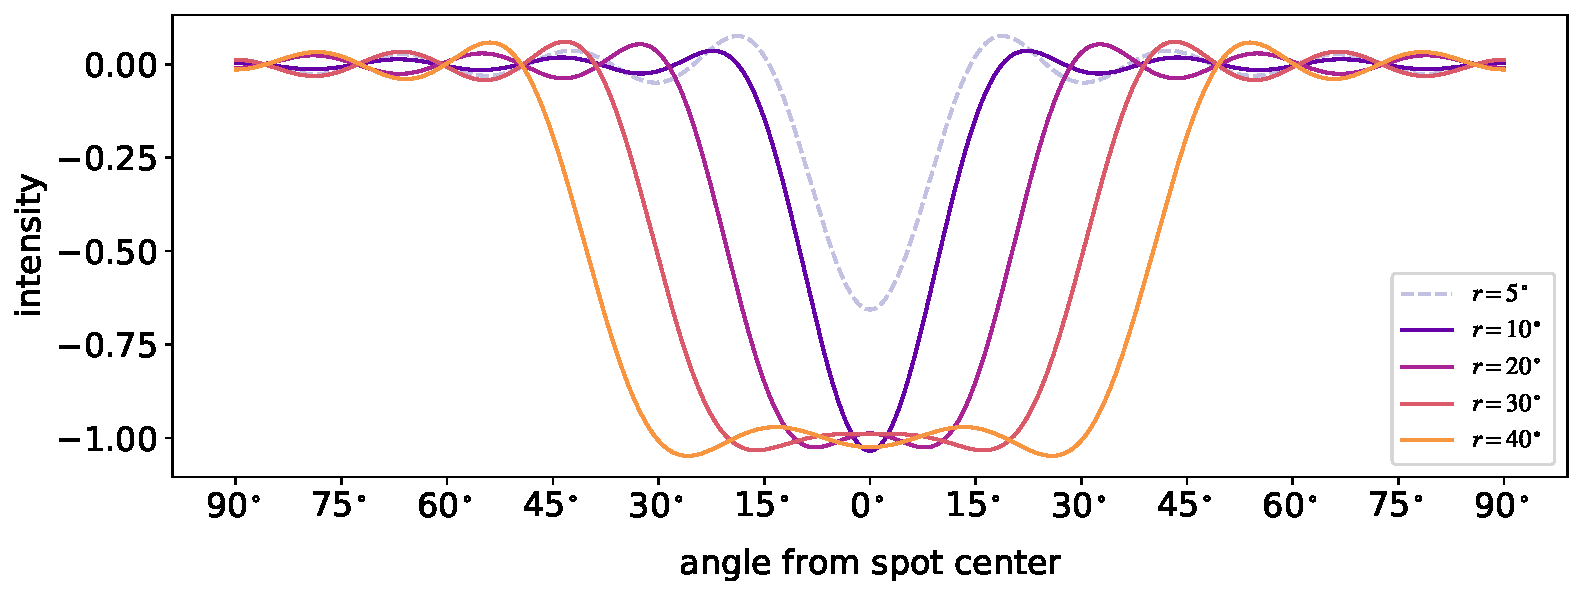
\includegraphics[width=\linewidth]{figures/spot_profile.pdf}
        \oscaption{spot_profile}{%
            Intensity profiles for spots with different
            radii $\rho$ computed at spherical harmonic
            degree $l_{\mathrm{max}} = \LMAX$.
            For $\rho \gtrsim 10^\circ$, the spherical harmonic expansion
            captures the spot shape and intensity reasonably well,
            albeit with some ringing due to the truncated expansion.
            \label{fig:spot_profile}
        }
    \end{centering}
\end{figure}

Figure~\ref{fig:spot_profile} shows the intensity profile for spots of
different radii expanded to spherical harmonic degree $l_{\mathrm{max}} = \LMAX$.
The average intensity
within the spots is close to $-1$ and the half-widths at half-minimum are
equal to the spot radii, as expected.
The effect of ringing due to the truncated spherical harmonic expansion is
evident, although it is strongly suppressed compared to an expansion
without the smoothing term (i.e., $\sigma = \infty$). However, for
$\rho \lesssim 10^\circ$, an expansion to $l_{\mathrm{max}} = \LMAX$ is
insufficient to correctly model the spot, as can be seen from the
$\rho = 5^\circ$ profile (dashed curve). Expansions to higher spherical harmonic
degree allow one to model spots with radii smaller than $10^\circ$, although
at increased computational cost and potential numerical stability issues;
we discuss this point at length in \S\ref{sec:tiny-spots}.


\subsubsection{Probability density function}
%
For simplicity, we will adopt a uniform probability distribution for the
spot radius, characterized by a mean radius $r$ and a half-width $\Delta$:
%
\begin{align}
    p(\rho \, \big| \, \pmb{\theta}_{\rho})
     & =
    \begin{cases}
        \frac{1}{2\Delta} & r - \Delta \leq r \leq r + \Delta
        \\
        0                 & \mathrm{otherwise}
        \quad,
    \end{cases}
\end{align}
%
where the hyperparameters of the distribution are
%
\begin{align}
    \pmb{\theta}_\rho = \left(
    r \, \, \, \,
    \Delta \right)^\top
    \quad.
\end{align}
%
As we argue in the text, in practice it is often difficult to constrain the
moments of the radius distribution above the first (the mean). It is
therefore useful to also consider the limiting case of the radius distribution
as $\Delta \rightarrow 0$, in which case the PDF becomes
%
\begin{align}
    p(\rho \, \big| \, \pmb{\theta}_{\rho}, \Delta = 0)
     & =
    \delta(\rho - r)
    \quad,
\end{align}
%
where $\delta$ is the delta function.
%

\subsubsection{First moment}
%
The first moment of the radius distribution is (Equation~\ref{eq:e1})
%
\begin{align}
    \mathbf{e}_\rho
     & \equiv
    \int
    \mathbf{s}(\rho) \,
    p(\rho \, \big| \, \pmb{\theta}_{\rho}) \,
    \mathrm{d}\rho
    \nonumber \\
     & =
    \frac{1}{2\Delta}
    \int_{r_0 - \Delta}^{r_0 + \Delta}
    \mathbf{s}(\rho) \,
    \mathrm{d}\rho
    \quad.
\end{align}
%
Using the equations from the previous section, its components may be written
%
\begin{align}
    (e_\rho)^l_m
     & =
    \frac{\delta_{m,0}}{2\Delta}
    \int_{r - \Delta}^{r+ \Delta}
    \tilde{s}_{l}(\rho) \,
    \mathrm{d}\rho
    \nonumber \\
     & =
    \frac{\delta_{m,0}}{2\Delta}
    \sum_{k=0}^{K-1} B^+_{l,k}
    \int_{r - \Delta}^{r + \Delta}
    b_{k}(\rho)
    \mathrm{d}\rho
    \nonumber \\
     & =
    \frac{\delta_{m,0} s}{2\Delta}
    \sum_{k=0}^{K-1} B^+_{l,k}
    \ln
    \left(
    \frac{
        1+\exp\left(\frac{r -\Delta -\vartheta_k}{s}\right)
    }
    {
        1+\exp\left(\frac{r + \Delta -\vartheta_k}{s}\right)
    }
    \right)
    \quad.
\end{align}
%
In the limit $\Delta \rightarrow 0$,
%
\begin{align}
    \lim_{\Delta \rightarrow 0}
    \mathbf{e}_\rho
     & =
    \mathbf{B}^+ \mathbf{b}(r)
    \quad.
\end{align}
%

\subsubsection{Second moment}
%
The second moment of the radius distribution is (Equation~\ref{eq:E1})
%
\begin{align}
    \mathbf{E}_\rho
     & \equiv
    \int
    \mathbf{s}(\rho) \,
    \mathbf{s}^\top(\rho) \,
    p(\rho \, \big| \, \pmb{\theta}_{\rho}) \,
    \mathrm{d}\rho
    \nonumber \\
     & =
    \frac{1}{2\Delta}
    \int_{r - \Delta}^{r + \Delta}
    \mathbf{s}(\rho) \,
    \mathbf{s}^\top(\rho) \,
    \mathrm{d}\rho
    \quad.
\end{align}
%
As before, its components may be written
%
%
\begin{align}
    (E_\rho)^{l,l'}_{m,m'}
     & =
    \frac{\delta_{m,0}\delta_{m',0}}{2\Delta}
    \int_{r - \Delta}^{r + \Delta}
    \tilde{s}^l_{m}(\rho) \,
    \tilde{s}^{l'}_{m'}(\rho) \,
    \mathrm{d}\rho
    \nonumber \\
     & =
    \frac{\delta_{m,0}\delta_{m',0}}{2\Delta}
    \sum_{k=0}^{K-1} B^+_{l,k}
    \sum_{k'=0}^{K-1} B^+_{l',k'}
    \int_{r - \Delta}^{r + \Delta}
    b_{k}(\rho)
    b_{k'}(\rho)
    \mathrm{d}\rho
    \nonumber \\
     & =
    \frac{\delta_{m,0}\delta_{m',0}s}{2\Delta}
    \sum_{k=0}^{K-1} B^+_{l,k}
    \sum_{k'=0}^{K-1} B^+_{l',k'}
    C_{k,k'}(r,\Delta)
    \quad,
\end{align}
%
where
%
\begin{align}
    C_{k,k'}(r,\Delta)
     & \equiv
    \frac{
        \exp\left(\frac{\vartheta_{k} - \vartheta_{k'}}{s}\right)
        \ln
        \left(
        \frac{
            1+\exp\left(\frac{r -\Delta -\vartheta_{k}}{s}\right)
        }
        {
            1+\exp\left(\frac{r + \Delta -\vartheta_{k}}{s}\right)
        }
        \right)
        -
        \ln
        \left(
        \frac{
            1+\exp\left(\frac{r -\Delta -\vartheta_{k'}}{s}\right)
        }
        {
            1+\exp\left(\frac{r + \Delta -\vartheta_{k'}}{s}\right)
        }
        \right)
    }{
        1
        -
        \exp\left(\frac{\vartheta_{k} - \vartheta_{k'}}{s}\right)
    }
    \quad.
\end{align}
%
In the limit $\Delta \rightarrow 0$,
%
\begin{align}
    \lim_{\Delta \rightarrow 0}
    \mathbf{E}_\rho
     & =
    \mathbf{B}^+ \mathbf{b}(r) \mathbf{b}^\top(r) {\mathbf{B}^+}^\top
    \quad.
\end{align}
%

\subsection{The Latitude Integrals}
\label{sec:lat}
%
Our goal in this section is to compute the first and second moments
of the latitude distribution ($\mathbf{e}_\phi$ and $\mathbf{E}_\phi$,
given by Equations \ref{eq:e2} and \ref{eq:E2}, respectively).
These involve integrals over the terms in the Wigner
rotation matrix for spherical harmonics, which we discuss below.

\subsubsection{Rotation matrices}
\label{sec:wigner}
%
The Wigner rotation matrix for real spherical harmonics up to degree $l_{\mathrm{max}}$
may be written as the block-diagonal matrix
%
\begin{align}
    \setstackgap{L}{1.25\baselineskip}
    \fixTABwidth{T}
    \mathbf{R} =
    \parenMatrixstack{
    \quad\quad \, \mathbf{R}^0 \, \quad\quad
     &              &              &        &                               \\
     & \mathbf{R}^1 &              &        &                               \\
     &              & \mathbf{R}^2 &        &                               \\
     &              &              & \ddots &                               \\
     &              &              &        & \mathbf{R}^{l_{\mathrm{max}}}
    }\quad,
\end{align}
%
where
%
\begin{align}
    \mathbf{R}^l = {\mathbf{U}^l}^{-1} \mathbf{D}^l \mathbf{U}^l
\end{align}
%
is the Wigner rotation matrix for a single spherical harmonic degree,
%
\begin{align}
    \label{eq:U}
    \setstackgap{L}{1.25\baselineskip}
    \fixTABwidth{T}
    \mathbf{U}^l =
    \frac{1}{\sqrt{2}}
    \parenMatrixstack{
        \quad\quad\, \ddots \, \quad\quad\quad\quad
           &       &        &       &          &    &   &    & \Ddots \\
           & \imag &        &       &          &    &   & 1  &        \\
           &       & \imag  &       &          &    & 1 &    &        \\
           &       &        & \imag &          & 1  &   &    &        \\
           &       &        &       & \sqrt{2} &    &   &    &        \\
           &       &        & \imag &          & -1 &   &    &        \\
           &       & -\imag &       &          &    & 1 &    &        \\
           & \imag &        &       &          &    &   & -1 &        \\
    \Ddots &       &        &       &          &    &   &    & \ddots
    }
\end{align}
%
describes the transformation from complex to real spherical harmonics,
and $\mathbf{D}$ is the Wigner matrix for complex spherical harmonics,
whose terms are given by the expression
%
\begin{align}
    D_{m,m'}^l(\alpha, \beta, \gamma) = \mathrm{e}^{-\imag m' \alpha}
    d_{m,m'}^l(\beta) \mathrm{e}^{-\imag m \gamma}
\end{align}
%
where $\alpha$, $\beta$, and $\gamma$ are the Euler angles describing
the rotation in the
$\hat{\mathbf{z}}{-}\hat{\mathbf{y}}{-}\hat{\mathbf{z}}$ convention
and $\imag$ is the imaginary unit. The terms of the $d$-matrix
depend on powers of $\sin\left(\nicefrac{\beta}{2}\right)$
and $\cos\left(\nicefrac{\beta}{2}\right)$
\citep[c.f. Equation C15 in][]{Luger2019}, but it is convenient to use
the half-angle formula to express these terms instead as
%
\begin{proof}{test_dlmmp}
    d_{m,m'}^l(\beta) =
    \sum\limits_{i=0}^{2l} c_{m,m',i}^{l}
    \mathrm{sgn}(\sin\beta)^{i}
    (1 - \cos\beta)^{\frac{2l - i}{2}}
    (1 + \cos\beta)^\frac{i}{2}
\end{proof}
%
where
%
\begin{proof}{test_dlmmp}
    c_{m,m',i}^{l} & =
    \resizebox{.75\hsize}{!}{$
            \begin{cases}
                \dfrac{
                \left(-1\right)^{\frac{2l + 3m + m' - i}{2}}
                \sqrt{\left(l - m\right)!
                    \left(l + m\right)!
                    \left(l - m'\right)!
                    \left(l + m'\right)!}
                }{
                2^l
                \left(\frac{i - m - m'}{2}\right)!
                \left(\frac{i + m + m'}{2}\right)!
                \left(\frac{2l - i - m + m'}{2}\right)!
                \left(\frac{2l - i + m - m'}{2}\right)!
                }
                %
                 & m - m' - i \,\, \mathrm{even}
                %
                \\[0.5em]
                0
                %
                 & m - m' - i \,\, \mathrm{odd}
            \end{cases}
        $}
\end{proof}
%

\subsubsection{Probability density function}
%
The latitude integrals (Equations~\ref{eq:e2} and \ref{eq:E2}) involve
rotations by an angle $\phi$ about $\hat{\mathbf{x}}$, which
may be accomplished by choosing
Euler angles $\alpha = \nicefrac{\pi}{2}$, $\beta = \phi$, and
$\gamma = -\nicefrac{\pi}{2}$, such that
%
\begin{align}
    \mathbf{R}^l_{\hat{\mathbf{x}}}(\phi)
     & =
    {\mathbf{U}^l}^{-1} \mathbf{D}^l_{\hat{\mathbf{x}}}(\phi) \mathbf{U}^l
\end{align}
%
with
\begin{align}
    \mathbf{D}^l_{\hat{\mathbf{x}}}(\phi)
     & =
    \mathbf{D}^l\left(\frac{\pi}{2}, \phi, -\frac{\pi}{2}\right)
    \quad.
\end{align}
%
From the expressions above, it is clear that all terms in
$\mathbf{R}_{\hat{\mathbf{x}}}(\phi)$ are equal to (weighted) sums of powers
of $(1 \pm \cos\phi)$.
%
Since our goal is to compute integrals of these terms multiplied by
a probability density function, it is convenient to model
$\cos\phi$ as a Beta-distributed variable. As we will see, this
choice will allow us to
analytically compute the first two moments of the distribution of
$\phi$ conditioned on $\pmb{\theta}_\phi$.

%
The Beta distribution in $\cos\phi$ has hyperparameters $\alpha$ and $\beta$
and PDF given by
%
\begin{align}
    \label{eq:cosphi-pdf}
    p \big(\cos\phi \, \big| \, \alpha, \beta \big)
     & =
    \dfrac{\Gamma(\alpha + \beta)}{\Gamma(\alpha)\Gamma(\beta)}
    (\cos\phi)^{\alpha - 1}
    (1 - \cos\phi)^{\beta - 1}
    \quad,
\end{align}
%
where $\Gamma$ is the Gamma function. The implied distribution for $\phi$
may be computed by a straightforward change of variable:
%
\begin{proof}{test_beta_transform}
    \label{eq:phi-pdf}
    p \big(\phi \, \big| \, \alpha, \beta \big)
    & =
    \dfrac{\Gamma(\alpha + \beta)}{2\Gamma(\alpha)\Gamma(\beta)}
    \big|
    \sin\phi
    \big|
    (\cos\phi)^{\alpha - 1}
    (1 - \cos\phi)^{\beta - 1}
    \quad,
\end{proof}
%
for $\phi \in \left[ -\frac{\pi}{2}, \frac{\pi}{2} \right]$.
%
Both $\alpha$ and $\beta$ are restricted to $(0, \infty)$.
However, in practice it is necessary to limit the values of these parameters
to a finite range to ensure the numerical stability of the algorithm.
It is also convenient
to work with the log of these quantities because of their large dynamic range.
We therefore introduce the modified shape parameters
%
\begin{align}
    \label{eq:gauss2beta}
    a & \equiv \frac{\ln\alpha - K_{00}}{K_{10} - K_{00}}
    \nonumber                                             \\[0.5em]
    b & \equiv \frac{\ln\beta - K_{10}}{K_{11} - K_{10}}
\end{align}
%
with inverse transform
%
\begin{align}
    \label{eq:beta2gauss}
    \alpha & = e^{K_{00} + (K_{10} - K_{00})a}
    \nonumber                                  \\
    \beta  & = e^{K_{10} + (K_{11} - K_{10})b}
    \quad,
\end{align}
%
where the matrix
%
\begin{align}
    \setstackgap{L}{1.25\baselineskip}
    \fixTABwidth{T}
    \mathbf{K}
    =
    \parenMatrixstack{
    0              & 5 \\
    \ln\frac{1}{2} & 5
    }
\end{align}
%
defines the minimum and maximum values of $\ln\alpha$ (top row) and $\ln\beta$
(bottom row) we adopt in our implementation of the algorithm. The lower limits
correspond to $\alpha > 1$ and $\beta > \frac{1}{2}$, which excludes
distributions with unphysically sharp peaks at $\phi = 90^\circ$. Both $a$
and $b$ are restricted to the domain $(0, 1)$, and together comprise the
hyperparameter vector
%
\begin{align}
    \pmb{\theta}_\phi = \left(
    a \, \, \, \,
    b \right)^\top
    \quad.
\end{align}
%

Although we use $a$ and $b$ as the inputs to our algorithm, below
we derive expressions for the moments of the distribution in terms
of $\alpha$ and $\beta$, as this is somewhat more convenient. Note that
this requires us to explicitly add a Jacobian term to the likelihood
when doing posterior inference to account for the change in volume due
to the transformation from $\alpha, \beta$ to $a, b$. In practice, however,
$\alpha$ and $\beta$ are no more natural a set of parameters to sample in,
since they do not \emph{obviously} relate to physical quantities of interest.
It is therefore desirable to introduce one final transform, from $\alpha, \beta$
to parameters controlling the mean (or mode) $\mu_\phi$ and
standard deviation  $\sigma_\phi$ of the
distribution of spot latitudes, which \emph{are} of physical interest.
We introduce this transform, and the associated Jacobian for the complete
transform $\mu_\phi, \sigma_\phi \rightarrow a, b$,
in \S\ref{sec:lat-transform} below.

\subsubsection{First moment}
%
Since the Wigner matrices are block diagonal, we may evaluate the moments of the
distribution one spherical harmonic degree at a time. To that end, let us
write the first moment integral as
%
\begin{proof}{test_ephi}
    \mathbf{e}_\phi
    & \equiv
    \int
    \mathbf{R}_{\hat{\mathbf{x}}}(\phi) \,
    \mathbf{e}_r \,
    p(\phi \, \big| \, \pmb{\theta}_{\phi}) \,
    \mathrm{d}\phi
    \nonumber
    \\
    %
    & =
    %
    \left(
    \mathbf{e}_\phi^0
    \,\,\,
    \mathbf{e}_\phi^1
    \,\,\,
    \mathbf{e}_\phi^2
    \,\,\,
    \cdots
    \,\,\,
    \mathbf{e}_\phi^{l_{\mathrm{max}}}
    \right)^\top
    \quad,
\end{proof}
%
where
%
\begin{proof}{test_ephi}
    \mathbf{e}_\phi^l
    & =
    \int
    \mathbf{R}^l_{\hat{\mathbf{x}}}(\phi) \,
    \mathbf{e}^l_r \,
    p(\phi \, \big| \, \pmb{\theta}_{\phi}) \,
    \mathrm{d}\phi
    \nonumber \\
    %
    & =
    %
    {\mathbf{U}^l}^{-1}
    \mathbf{p}^l_\phi
    \quad,
\end{proof}
%
and we define
%
\begin{align}
    \label{eq:plphi}
    \mathbf{p}^l_\phi
     & \equiv
    \int
    \mathbf{D}^l_{\hat{\mathbf{x}}}(\phi) \,
    \bar{\mathbf{e}}^l_r \,
    p(\phi \, \big| \, \pmb{\theta}_{\phi}) \,
    \mathrm{d}\phi
    \\
    \bar{\mathbf{e}}^l_r
     & \equiv
    \mathbf{U}^l
    \mathbf{e}^l_r
    \quad.
\end{align}
%
The integral $\mathbf{p}_\phi^l$ defined above has a closed-form solution.
To show this, we write the terms of $\mathbf{p}^l_\phi$ as
%
\begin{align}
    {({p^l_\phi})_{}}_m
     & =
    \int
    \sum\limits_{\mu=-l}^l
    {({D^l_{\hat{\mathbf{x}}}})_{}}_{m,\mu}(\phi) \,
    {({\bar{e}}^l_r)_{}}_{\mu} \,
    p(\phi \, \big| \, \pmb{\theta}_{\phi}) \,
    \mathrm{d}\phi
    %
    \nonumber \\[0.5em]
    %
     & =
    \dfrac{\Gamma(\alpha + \beta)}{\Gamma(\alpha)\Gamma(\beta)}
    \sum\limits_{\mu=-l}^l
    {({\bar{e}}^l_r)_{}}_{\mu}
    \mathrm{e}^{\frac{\imag \pi}{2}(m - \mu)}
    \sum\limits_{i=0}^{2l} c_{m,\mu,i}^{l}
    \,
    {({q^l_\phi})_{}}_i(\pmb{\theta}_{\phi})
    \quad,
\end{align}
%
where
%
\begin{proof}{test_qlphii}
    {({q^l_\phi})_{}}_i(\pmb{\theta}_{\phi})
    & \equiv
    \frac{1}{2}
    \int_{-\frac{\pi}{2}}^{\frac{\pi}{2}}
    %
    \mathrm{sgn}(\sin\phi)^{i}
    \big| \sin\phi \big|
    (\cos\phi)^{\alpha - 1}
    (1 - \cos\phi)^{l + \beta - \frac{i}{2} - 1}
    (1 + \cos\phi)^\frac{i}{2}
    %
    \,
    \mathrm{d}\phi
    \nonumber \\[0.5em]
    %
    & =
    %
    \begin{cases}
        \displaystyle\int_{0}^{1}
        %
        x^{\alpha - 1}
        (1 - x)^{l + \beta - \frac{i}{2} - 1 }
        (1 + x)^\frac{i}{2}
        %
        \,
        \mathrm{d}x
        %
         & i \,\, \mathrm{even}
        %
        \\
        %
        0
        %
         & i \,\, \mathrm{odd} \quad,
    \end{cases}
\end{proof}
%
and in the last line we made use of the transformation $x = \cos\phi$.
%
The integral in the expression above has a closed-form solution in terms
of the hypergeometric function $_2F_1$:
%
\begin{proof}{test_qlphii}
    %
    \label{eq:qlphii}
    {({q^l_\phi})_{}}_i(\pmb{\theta}_{\phi})
    & =
    \resizebox{.75\hsize}{!}{$
            \begin{cases}
                \dfrac{\Gamma(\alpha)\Gamma(l + \beta - \frac{i}{2})}{\Gamma(l + \alpha + \beta - \frac{i}{2})}
                \,
                _2F_1\Big(
                -\frac{i}{2},
                \alpha;
                l + \alpha + \beta - \frac{i}{2};
                -1
                \Big)
                %
                 & i \,\, \mathrm{even}
                %
                \\
                %
                0
                %
                 & i \,\, \mathrm{odd} \quad.
            \end{cases}
        $}
\end{proof}
%
In order to compute the integral $\mathbf{e}_\phi$
(Equation~\ref{eq:e2}) we must evaluate Equation~(\ref{eq:qlphii})
for all $0 \leq l \leq l_{\mathrm{max}}$, $0 \leq i \leq 2l$,
which can be done efficiently via upward recursion relations for both
the gamma function and the hypergeometric function.

\subsubsection{Second moment}
%
Similarly as before, let us write the second moment integral as
%
\begin{proof}{}
    \label{eq:Ephi}
    \mathbf{E}_\phi
    & \equiv
    \int
    \mathbf{R}_{\hat{\mathbf{x}}}(\phi) \,
    \mathbf{E}_r \,
    \mathbf{R}_{\hat{\mathbf{x}}}^\top(\phi) \,
    p(\phi \, \big| \, \pmb{\theta}_{\phi}) \,
    \mathrm{d}\phi
    \nonumber
    \\
    %
    & =
    %
    \setstackgap{L}{1.25\baselineskip}
    \fixTABwidth{T}
    \parenMatrixstack{
    \mathbf{E}_\phi^{0,0} & \mathbf{E}_\phi^{0,1} & \mathbf{E}_\phi^{0,2} & \cdots & \mathbf{E}_\phi^{0,l_{\mathrm{max}}} \\
    \mathbf{E}_\phi^{1,0} & \mathbf{E}_\phi^{1,1} & \mathbf{E}_\phi^{1,2} & \cdots & \mathbf{E}_\phi^{1,l_{\mathrm{max}}} \\
    \mathbf{E}_\phi^{2,0} & \mathbf{E}_\phi^{2,1} & \mathbf{E}_\phi^{2,2} & \cdots & \mathbf{E}_\phi^{2,l_{\mathrm{max}}} \\
    \vdots & \vdots & \vdots & \ddots & \vdots \\
    \mathbf{E}_\phi^{l_{\mathrm{max}},0} & \mathbf{E}_\phi^{l_{\mathrm{max}},1} & \mathbf{E}_\phi^{l_{\mathrm{max}},2} & \cdots & \mathbf{E}_\phi^{l_{\mathrm{max}},l_{\mathrm{max}}}
    }
    \quad,
\end{proof}
%
where
%
\begin{proof}{}
    \mathbf{E}_\phi^{l,l'}
    & =
    \int
    \mathbf{R}^l_{\hat{\mathbf{x}}}(\phi) \,
    \mathbf{E}^{l,l'}_r \,
    {\mathbf{R}^{l'}_{\hat{\mathbf{x}}}}^\top(\phi) \,
    p(\phi \, \big| \, \pmb{\theta}_{\phi}) \,
    \mathrm{d}\phi
    \nonumber \\
    %
    & =
    %
    {\mathbf{U}^l}^{-1}
    \mathbf{P}^{l,l'}_\phi
    {{\mathbf{U}^{l'}}^{-1}}^\top
\end{proof}
%
and we define
%
\begin{align}
    \label{eq:Plphi}
    \mathbf{P}^{l,l'}_\phi
     & \equiv
    \int
    \mathbf{D}^l_{\hat{\mathbf{x}}}(\phi) \,
    \bar{\mathbf{E}}^{l,l'}_r \,
    {\mathbf{D}^{l'}_{\hat{\mathbf{x}}}}^\top(\phi) \,
    p(\phi \, \big| \, \pmb{\theta}_{\phi}) \,
    \mathrm{d}\phi
    \\
    \bar{\mathbf{E}}^{l,l'}_r
     & \equiv
    \mathbf{U}^l
    \mathbf{E}^{l,l'}_r
    {\mathbf{U}^{l'}}^\top
    \quad.
\end{align}
%
As before, we may express the solution to the integral $\mathbf{P}^{l,l'}_\phi$ in
closed form. Let us write the terms of $\mathbf{P}^{l,l'}_\phi$ as
%
\begin{align}
    {({P^{l,l'}_\phi})_{}}_{m,m'}
     & =
    \int
    \sum\limits_{\mu=-l}^l
    \sum\limits_{{\mu'}=-l'}^{l'}
    {({D^l_{\hat{\mathbf{x}}}})_{}}_{m,\mu}(\phi) \,
    {(\bar{E}^{l,l'}_r)_{}}_{\mu,{\mu'}} \,
    {({D^{l'}_{\hat{\mathbf{x}}}})_{}}_{{\mu'},m'}(\phi) \,
    p(\phi \, \big| \, \pmb{\theta}_{\phi}) \,
    \mathrm{d}\phi
    %
    \nonumber \\[0.5em]
    %
     & =
    \resizebox{.75\hsize}{!}{$
        \dfrac{\Gamma(\alpha + \beta)}{\Gamma(\alpha)\Gamma(\beta)}
        \sum\limits_{\mu=-l}^l
        \sum\limits_{{\mu'}=-l'}^{l'}
        {(\bar{E}^{l,l'}_r)_{}}_{\mu,{\mu'}} \,
        \mathrm{e}^{\frac{\imag \pi}{2}(m - \mu + {\mu'} - m')}
        \sum\limits_{i=0}^{2l}
        \sum\limits_{i'=0}^{2l'}
        c_{m,\mu,i}^{l}
        c_{{\mu'},m',i'}^{l'}
        \,
        {({Q^{l,l'}_\phi})_{}}_{i,i'}(\pmb{\theta}_{\phi})
    $}
    \quad,
\end{align}
%
where, similarly to before,
%
\begin{proof}{}
    {({Q^{l,l'}_\phi})_{}}_{i,i'}(\pmb{\theta}_{\phi})
    & \equiv
    \frac{1}{2}
    \int_{-\frac{\pi}{2}}^{\frac{\pi}{2}}
    %
    \mathrm{sgn}(\sin\phi)^{i+i'}
    \big| \sin\phi \big|
    (\cos\phi)^{\alpha - 1}
    (1 - \cos\phi)^{l + l' + \beta - \frac{i+i'}{2} - 1}
    (1 + \cos\phi)^\frac{i+i'}{2}
    %
    \,
    \mathrm{d}\phi
    \nonumber \\[0.5em]
    %
    & =
    %
    \begin{cases}
        \displaystyle\int_{0}^{1}
        %
        x^{\alpha - 1}
        (1 - x)^{l + l' + \beta - \frac{i+i'}{2} - 1 }
        (1 + x)^\frac{i+i'}{2}
        %
        \,
        \mathrm{d}x
        %
         & i+i' \,\, \mathrm{even}
        %
        \\
        %
        0
        %
         & i+i' \,\, \mathrm{odd} \quad.
    \end{cases}
\end{proof}
%
We may again express this integral in closed form:
%
\begin{proof}{}
    %
    \label{eq:Qlphiij}
    {({Q^{l,l'}_\phi})_{}}_{i,i'}(\pmb{\theta}_{\phi})
    & =
    \resizebox{.75\hsize}{!}{$
            \begin{cases}
                \dfrac{\Gamma(\alpha)\Gamma(l + l' + \beta - \frac{i+i'}{2})}{\Gamma(l + l' + \alpha + \beta - \frac{i+i'}{2})}
                \,
                _2F_1\Big(
                -\frac{i+i'}{2},
                \alpha;
                l + l' + \alpha + \beta - \frac{i+i'}{2};
                -1
                \Big)
                %
                 & i+i' \,\, \mathrm{even}
                %
                \\
                %
                0
                %
                 & i+i' \,\, \mathrm{odd} \quad.
            \end{cases}
        $}
\end{proof}
%
As before, this integral may be evaluated recursively to efficiently compute all
of the terms in $\mathbf{E}_\phi$.

\subsubsection{Variable transforms}
\label{sec:lat-transform}

As we mentioned earlier,
although we adopt $a$ and $b$ as the actual inputs to our Gaussian process
(i.e., as elements of the input vector $\pmb{\theta}_\bullet$), these
parameters are not themselves ``interpretable'', as they do not directly
correspond to physical
quantities of interest such as the mean and standard deviation of the spot
latitude distribution. However, over most of the parameter space in $a$ and $b$,
the spot latitude distribution is well approximated
by a bimodal Gaussian. In particular, there exists
a one-to-one relationship between $a$ and $b$ and the mean $\mu_\phi$
and standard deviation $\sigma_\phi$ of a normal approximation to the
distribution. Moreover, we find that
if we let $\mu_\phi$ be the \emph{mode} of the PDF and
$\sigma_\phi^2$ be a \emph{local} approximation to the variance of the PDF,
the relationship has a convenient closed form.

To compute $\mu_\phi$, we differentiate Equation~(\ref{eq:phi-pdf}) with respect
to $\phi$, set the expression equal to zero, and solve
for $\phi$ to obtain
%
\begin{proof}{}
    \mu_\phi &= 2 \tan^{-1}
    \left(
    \sqrt{
        2 \alpha + \beta - 2 -
        \sqrt{
            4 \alpha^2
            - 8 \alpha
            - 6 \beta
            + 4 \alpha \beta
            + \beta^2
            + 5
        }
    }
    \right)
\end{proof}
%
where $\alpha$ and $\beta$ may be computed from $a$ and $b$ via
Equation~(\ref{eq:beta2gauss}).
%
To compute $\sigma_\phi$, we note that the variance of a Gaussian distribution
$\varphi(\phi)$
is the negative reciprocal of its curvature in log space:
%
\begin{align}
    \sigma^2 = -\left(\frac{\mathrm{d}^2 \ln \varphi(\phi)}{\mathrm{d}\phi^2}\right)^{-1}
\end{align}
%
We therefore twice differentiate the log of Equation~(\ref{eq:phi-pdf}), negate it,
take the reciprocal, and evaluate it at $\phi = \mu_\phi$ to obtain a local
approximation to the standard deviation of the distribution at the mode:
%
\begin{proof}{}
    \sigma_\phi &= \frac{\sin\mu_\phi}{
        \sqrt{1
            - \alpha
            + \beta
            + \left(\beta - 1\right) \cos\mu_\phi
            + \dfrac{\alpha - 1}{\cos\mu_\phi^2}}}
    \quad.
\end{proof}
%
For completeness, the inverse transform also has a closed form:
%
\begin{proof}{}
    \alpha &= \frac{2 + 4 \sigma_\phi^2 + (3 + 8 \sigma_\phi^2) \cos\mu_\phi + 2 \cos\left( 2\mu_\phi \right) + \cos\left( 3\mu_\phi \right)}{16 \sigma_\phi^2 \cos\left( \frac{\mu_\phi}{2} \right)^4} \\
    \beta &= \frac{\cos\mu_\phi + 2 \sigma_\phi^2 (3 + \cos\left( 2\mu_\phi \right)) - \cos\left( 3\mu_\phi \right)}{16 \sigma_\phi^2 \cos\left( \frac{\mu_\phi}{2} \right)^4}
    \quad.
\end{proof}

These transformations allow one to easily transform constraints on $a$ and
$b$ to constraints on the mode and approximate variance of the distribution
of spot latitudes. Importantly, they also allow us to compute the Jacobian
of the transform, given by
%
\begin{proof}{}
    J &=
    \frac{\partial{\mu_\phi}}{\partial{a}}
    \frac{\partial{\sigma_\phi}}{\partial{b}} -
    \frac{\partial{\mu_\phi}}{\partial{b}}
    \frac{\partial{\sigma_\phi}}{\partial{a}}
    %
    \\
    %
    &=\resizebox{.925\hsize}{!}{$
            \frac{
                \alpha \beta \left(1 + \cos\mu_\phi\right)^3
                \sin\left(2\mu_\phi\right)^3
            }{
                \sigma_\phi
                \left(
                2 \alpha + \beta - 3 +
                \left(2 \alpha + \beta - 1\right) \cos\mu_\phi
                \right)
                \left(
                2 \left( \alpha + \beta - 1\right) +
                3 (\beta - 1) \cos\mu_\phi
                - 2 \left( \alpha - \beta - 1 \right) \cos\left( 2\mu_\phi \right)
                + \left( \beta - 1\right) \cos\left( 3\mu_\phi \right)
                \right)^2
            }
        $}
    \nonumber
\end{proof}
%
While one could sample in $\mu_\phi$ and $\sigma_\phi$ directly, we instead
recommend sampling in the quantities $a$ and $b$ under a uniform prior on
$(0, 1)$ for both of them, then correcting for the implied prior on
$\mu_\phi$ and $\sigma_\phi$ by adding the log of the absolute value of $J$ to the log
likelihood. This corrects for the \emph{ad hoc}
prior on the latitude parameters introduced by our particular choice of
parametrization, enforcing instead a uniform prior on the quantities $\mu_\phi$
and $\sigma_\phi$.

\begin{figure}[ht!]
    \begin{centering}
        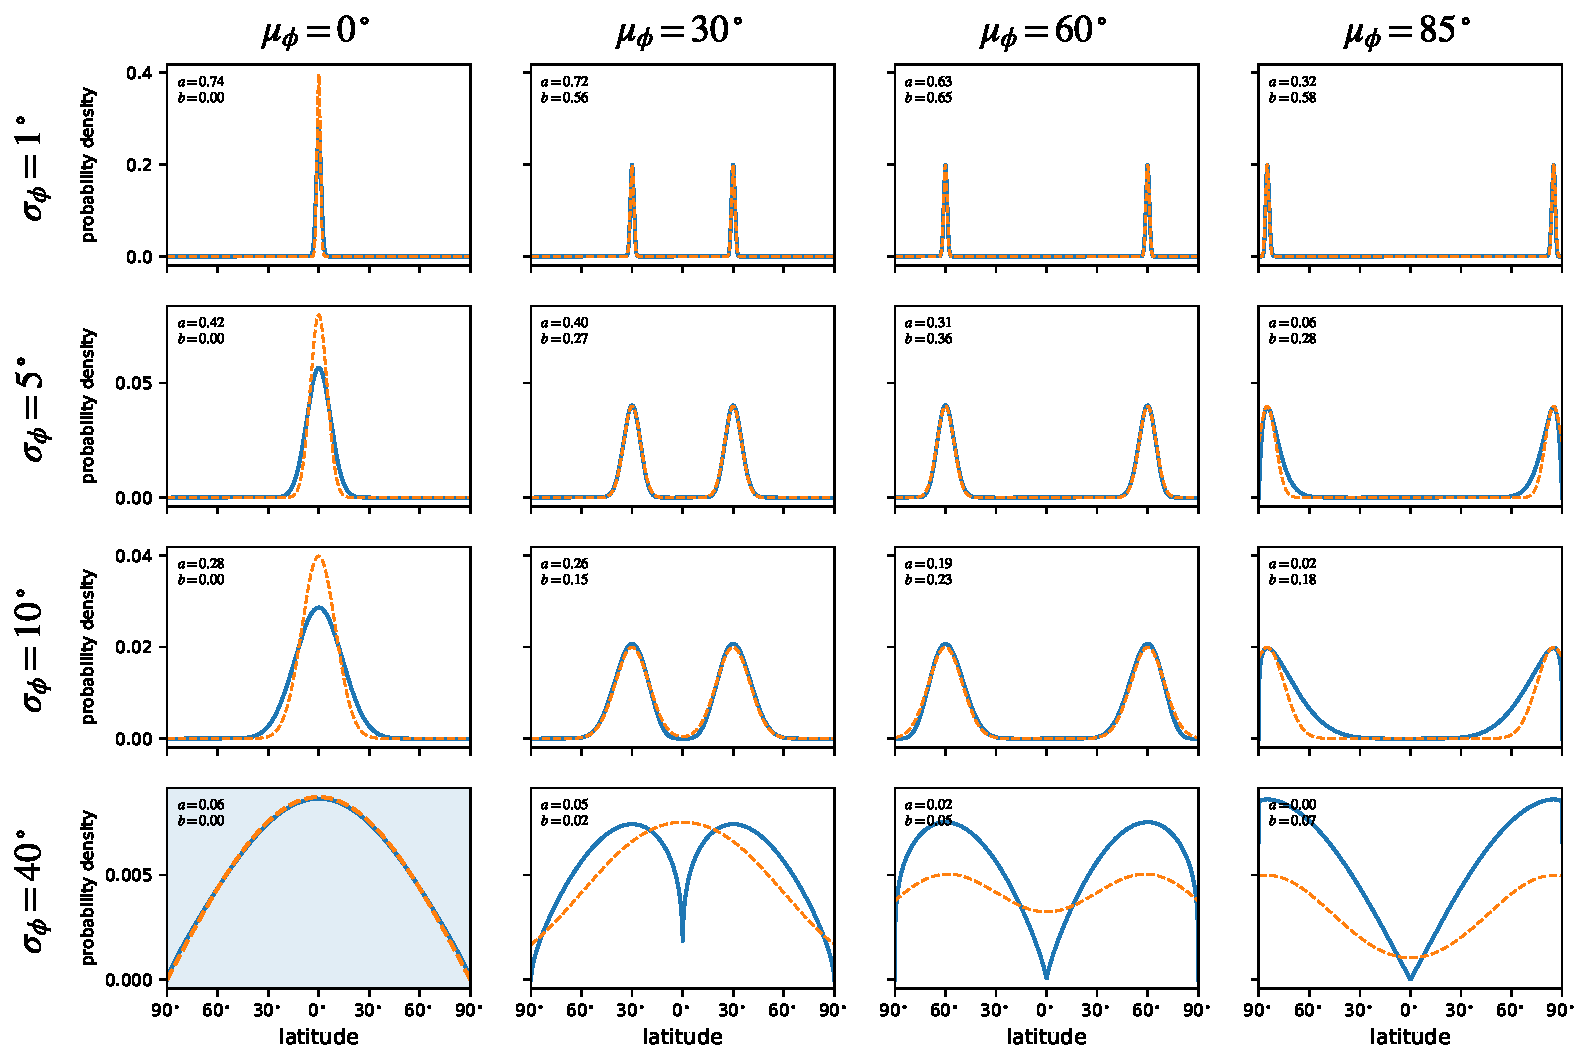
\includegraphics[width=\linewidth]{figures/latitude_pdf.pdf}
        \oscaption{latitude_pdf}{%
            Probability density function for the spot latitude (blue curves)
            for different values of the mode $\mu_\phi$ (columns)
            and local standard deviation $\sigma_\phi$ (rows).
            The corresponding values of $a$ and $b$ are
            indicated within each panel. The bimodal
            normal distribution with mean $\mu_\phi$ and standard deviation
            $\sigma_\phi$ is shown as the dashed orange curves; for mid-latitude
            modes and low standard deviations, the Gaussian approximation is
            quite good.
            The shaded panel in the lower right
            ($\mu_\phi = 0^\circ$, $\sigma_\phi = 0^\circ$)
            corresponds to an approximately isotropic distribution of
            spots over the surface of the star; in this panel only, the
            dashed orange curve corresponds to a cosine distribution in
            $\phi$ (i.e., the exact isotropic distribution).
            \label{fig:latitude_pdf}
        }
    \end{centering}
\end{figure}

For reference, Figure~\ref{fig:latitude_pdf} shows the latitude PDF
and the corresponding Gaussian approximation for different values of
$\mu_\phi$ and $\sigma_\phi$. The corresponding values of $a$ and $b$ are
indicated in the top left of each panel. For $\mu_\phi$ at intermediate
latitudes and moderate values of $\sigma_\phi$, the approximation is quite good.
However, for $\mu_\phi$ very close to the equator or to the poles, the curvature of
the distribution changes significantly as a function of $\phi$, so the variance is somewhat
underestimated by the approximation; and for $\sigma_\phi$ large, the
distribution becomes noticeably non-Gaussian.

The shaded panel at the lower left is a special case of the distribution
($\mu_\phi = 0^\circ$, $\sigma_\phi \approx 40^\circ$; or equivalently,
$a \approx 0.06$, $b = 0$), which is approximately isotropic in latitude. In
this panel, the orange curve instead corresponds to an isotropic (cosine)
distribution in $\phi$; note the excellent agreement.

Thus, in addition to having closed-form moments, the Beta distribution is
quite flexible and, via the transforms outlined above, intuitive in how
it affects the distribution of spots on the surface of a star.

\subsection{The Longitude Integrals}
\label{sec:lon}

In this section we will compute the first and second moments
of the longitude distribution
($\mathbf{e}_\lambda$ and $\mathbf{E}_\lambda$, given by Equations
\ref{eq:e3} and \ref{eq:E3}, respectively). The math here is
very similar to that in the previous section, as we are again
dealing with integrals of Wigner matrices (\S\ref{sec:wigner}).

\subsubsection{Probability density function}
%
The longitude integrals (Equations~\ref{eq:e3} and \ref{eq:E3}) involve
rotations by an angle $\lambda$ about $\hat{\mathbf{y}}$, which
may be accomplished by choosing
Euler angles $\alpha = 0$, $\beta = \lambda$, and
$\gamma = 0$, such that
%
\begin{align}
    \mathbf{R}^l_{\hat{\mathbf{y}}}(\lambda)
     & =
    {\mathbf{U}^l}^{-1} \mathbf{D}^l_{\hat{\mathbf{y}}}(\lambda) \mathbf{U}^l
\end{align}
%
with
\begin{align}
    \mathbf{D}^l_{\hat{\mathbf{y}}}(\lambda)
     & =
    \mathbf{D}^l\left(0, \lambda, 0\right)
    \quad.
\end{align}
%
Since we expect the longitudinal distribution of features on the surfaces
of stars to be (on average) isotropic, we will place a uniform prior on
$\lambda \in [-\pi, \pi)$:
%
\begin{align}
    p(\lambda \big| \pmb{\theta}_\lambda)
     & =
    \begin{cases}
        \frac{1}{2\pi} & -\pi \leq \lambda < \pi
        \\
        0              & \mathrm{otherwise} \quad.
    \end{cases}
\end{align}
%
We therefore have no hyperparameters
controlling the longitudinal distribution, i.e.,
%
\begin{align}
    \pmb{\theta}_\lambda = \left( \,\,\, \right)
    \quad.
\end{align}
%

\subsubsection{First moment}
%
As before, we will solve for the terms of the moment integrals one
spherical harmonic degree at a time:
%
\begin{proof}{test_elam}
    \mathbf{e}_\lambda
    & \equiv
    \int
    \mathbf{R}_{\hat{\mathbf{y}}}(\lambda) \,
    \mathbf{e}_\phi \,
    p(\lambda \, \big| \, \pmb{\theta}_{\lambda}) \,
    \mathrm{d}\lambda
    \nonumber
    \\
    %
    & =
    %
    \left(
    \mathbf{e}_\lambda^0
    \,\,\,
    \mathbf{e}_\lambda^1
    \,\,\,
    \mathbf{e}_\lambda^2
    \,\,\,
    \cdots
    \,\,\,
    \mathbf{e}_\lambda^{l_{\mathrm{max}}}
    \right)^\top
    \quad,
\end{proof}
%
where
%
\begin{proof}{test_elam}
    \mathbf{e}_\lambda^l
    & =
    \int
    \mathbf{R}^l_{\hat{\mathbf{y}}}(\lambda) \,
    \mathbf{e}^l_\phi \,
    p(\lambda \, \big| \, \pmb{\theta}_{\lambda}) \,
    \mathrm{d}\lambda
    \nonumber \\
    %
    & =
    %
    {\mathbf{U}^l}^{-1}
    \mathbf{p}^l_\lambda
    \quad,
\end{proof}
%
and we define
%
\begin{align}
    \label{eq:pllam}
    \mathbf{p}^l_\lambda
     & \equiv
    \int
    \mathbf{D}^l_{\hat{\mathbf{x}}}(\lambda) \,
    \bar{\mathbf{e}}^l_\phi \,
    p(\lambda \, \big| \, \pmb{\theta}_{\lambda}) \,
    \mathrm{d}\lambda
    \\
    \bar{\mathbf{e}}^l_\phi
     & \equiv
    \mathbf{U}^l
    \mathbf{e}^l_\phi
    \quad.
\end{align}
%
The integral $\mathbf{p}^l_\lambda$ defined above has a closed-form solution.
To show this, we write the terms of $\mathbf{p}^l_\lambda$ as
%
\begin{align}
    {({p^l_\lambda})_{}}_m
     & =
    \int
    \sum\limits_{\mu=-l}^l
    {({D^l_{\hat{\mathbf{y}}}})_{}}_{m,\mu}(\lambda) \,
    {({\bar{e}^l_\phi})_{}}_{\mu} \,
    p(\lambda \, \big| \, \pmb{\theta}_{\lambda}) \,
    \mathrm{d}\lambda
    %
    \nonumber \\[0.5em]
    %
     & =
    \sum\limits_{\mu=-l}^l
    {({\bar{e}^l_\phi})_{}}_{\mu} \,
    \sum\limits_{i=0}^{2l} c_{m,\mu,i}^{l}
    \,
    {({q^l_\lambda})_{}}_i
    \quad,
\end{align}
%
where
%
\begin{proof}{test_qllam}
    {({q^l_\lambda})_{}}_i
    & \equiv
    \frac{1}{2\pi}
    \int_{-\pi}^{\pi}
    %
    \mathrm{sgn}(\sin\lambda)^{i}
    (1 - \cos\lambda)^{l - \frac{i}{2}}
    (1 + \cos\lambda)^\frac{i}{2}
    %
    \,
    \mathrm{d}\lambda
    \nonumber \\[0.5em]
    %
    & =
    %
    \begin{cases}
        \dfrac{2^l \Gamma \left(\frac{1+i}{2}\right)
            \Gamma \left(l+\frac{1-i}{2}\right)}{\pi  \Gamma (l+1)}
        %
         & i \,\, \mathrm{even}
        %
        \\
        %
        0
        %
         & i \,\, \mathrm{odd} \quad,
    \end{cases}
\end{proof}
%
whose terms may easily be computed by upward recursion.
Since $\mathbf{q}^l_I$ does not depend on any user inputs,
it may be computed a single time as a pre-processing step
for efficiency.

\subsubsection{Second moment}
%
We write the second moment integral as
%
\begin{proof}{}
    \mathbf{E}_\lambda
    & \equiv
    \int
    \mathbf{R}_{\hat{\mathbf{y}}}(\lambda) \,
    \mathbf{E}_\phi \,
    \mathbf{R}_{\hat{\mathbf{y}}}^\top(\lambda) \,
    p(\lambda \, \big| \, \pmb{\theta}_{\lambda}) \,
    \mathrm{d}\lambda
    \nonumber
    \\
    %
    & =
    %
    \setstackgap{L}{1.25\baselineskip}
    \fixTABwidth{T}
    \parenMatrixstack{
    \mathbf{E}_\lambda^{0,0} & \mathbf{E}_\lambda^{0,1} & \mathbf{E}_\lambda^{0,2} & \cdots & \mathbf{E}_\lambda^{0,l_{\mathrm{max}}} \\
    \mathbf{E}_\lambda^{1,0} & \mathbf{E}_\lambda^{1,1} & \mathbf{E}_\lambda^{1,2} & \cdots & \mathbf{E}_\lambda^{1,l_{\mathrm{max}}} \\
    \mathbf{E}_\lambda^{2,0} & \mathbf{E}_\lambda^{2,1} & \mathbf{E}_\lambda^{2,2} & \cdots & \mathbf{E}_\lambda^{2,l_{\mathrm{max}}} \\
    \vdots & \vdots & \vdots & \ddots & \vdots \\
    \mathbf{E}_\lambda^{l_{\mathrm{max}},0} & \mathbf{E}_\lambda^{l_{\mathrm{max}},1} & \mathbf{E}_\lambda^{l_{\mathrm{max}},2} & \cdots & \mathbf{E}_\lambda^{l_{\mathrm{max}},l_{\mathrm{max}}}
    }
    \quad,
\end{proof}
%
where
%
\begin{proof}{}
    \mathbf{E}_\lambda^{l,l'}
    & =
    \int
    \mathbf{R}^l_{\hat{\mathbf{y}}}(\lambda) \,
    \mathbf{E}^{l,l'}_\phi \,
    {\mathbf{R}^{l'}_{\hat{\mathbf{y}}}}^\top(\lambda) \,
    p(\lambda \, \big| \, \pmb{\theta}_{\lambda}) \,
    \mathrm{d}\lambda
    \nonumber \\
    %
    & =
    %
    {\mathbf{U}^l}^{-1}
    \mathbf{P}^{l,l'}_\lambda
    {{\mathbf{U}^{l'}}^{-1}}^\top
\end{proof}
%
and we define
%
\begin{align}
    \label{eq:Pllam}
    \mathbf{P}^{l,l'}_\lambda
     & \equiv
    \int
    \mathbf{D}^l_{\hat{\mathbf{x}}}(\lambda) \,
    \bar{\mathbf{E}}^{l,l'}_\phi \,
    {\mathbf{D}^{l'}_{\hat{\mathbf{x}}}}^\top(\lambda) \,
    p(\lambda \, \big| \, \pmb{\theta}_{\lambda}) \,
    \mathrm{d}\lambda
    \\
    \bar{\mathbf{E}}^{l,l'}_\phi
     & \equiv
    \mathbf{U}^l
    \mathbf{E}^{l,l'}_\phi
    {\mathbf{U}^{l'}}^\top
    \quad.
\end{align}
%
We then express the terms of $\mathbf{P}^{l,l'}_\lambda$ as
%
\begin{align}
    {({P^{l,l'}_\lambda})_{}}_{m,m'}
     & =
    \int
    \sum\limits_{\mu=-l}^l
    \sum\limits_{{\mu'}=-l'}^{l'}
    ({D^l_{\hat{\mathbf{x}}}})_{m,\mu}(\lambda) \,
    (\bar{E}^{l,l'}_\phi)_{\mu,{\mu'}} \,
    ({D^{l'}_{\hat{\mathbf{x}}}})_{{\mu'},m'}(\lambda) \,
    p(\lambda \, \big| \, \pmb{\theta}_{\lambda}) \,
    \mathrm{d}\lambda
    %
    \nonumber \\[0.5em]
    %
     & =
    \sum\limits_{\mu=-l}^l
    \sum\limits_{{\mu'}=-l'}^{l'}
    (\bar{E}^{l,l'}_\phi)_{\mu,{\mu'}}
    \sum\limits_{i=0}^{2l}
    \sum\limits_{i'=0}^{2l'}
    c_{m,\mu,i}^{l}
    c_{{\mu'},m',i'}^{l'}
    \,
    (Q^{l,l'}_\lambda)_{i,i'}
    \quad,
\end{align}
%
where
%
\begin{proof}{}
    (Q^{l,l'}_\lambda)_{i,i'}
    & \equiv
    \frac{1}{2\pi}
    \int_{-\pi}^{\pi}
    %
    \mathrm{sgn}(\sin\lambda)^{i+i'}
    (1 - \cos\lambda)^{l + l' - \frac{i+i'}{2}}
    (1 + \cos\lambda)^\frac{i+i'}{2}
    %
    \,
    \mathrm{d}\lambda
    \nonumber \\[0.5em]
    %
    & =
    %
    \begin{cases}
        \dfrac{2^{l+l'} \Gamma \left(\frac{1+i+i'}{2}\right)
            \Gamma \left(l+l'+\frac{1-i-i'}{2}\right)}{\pi  \Gamma (l+l'+1)}
        %
         & i+i' \,\, \mathrm{even}
        %
        \\
        %
        0
        %
         & i+i' \,\, \mathrm{odd} \quad,
    \end{cases}
\end{proof}
%
whose terms may again be computed by upward recursion in a single
pre-processing step.


\subsection{The Contrast Integrals}
\label{sec:contrast}
%
The final integrals we must take in our computation of
$\mathrm{E} \big[ \mathbf{y} \, \big| \, \pmb{\theta}_\bullet \big]$
and $\mathrm{E} \big[ \mathbf{y} \mathbf{y}^\top \, \big| \, \pmb{\theta}_\bullet \big]$
are the integrals over
the spot contrast distribution, $\mathbf{e}_\xi$ and $\mathbf{E}_\xi$.
These are by far the easiest, since the spot contrast is a scalar
multiplier of the spherical harmonic coefficient vector, so we can
pull the terms $\mathbf{e}_\lambda$ and $\mathbf{E}_\lambda$ out
of the
integrals in Equations (\ref{eq:e4}) and (\ref{eq:E4}) to write
%
\begin{align}
    \mathbf{e}_\xi
     & \equiv
    \mathbf{e}_\lambda \,
    \int
    \xi \,
    p(\xi \, \big| \, \pmb{\theta}_{\xi}) \,
    \mathrm{d}\xi
    \\
    \mathbf{E}_\xi
     & \equiv
    \mathbf{E}_\lambda \,
    \int
    \xi^2 \,
    p(\xi \, \big| \, \pmb{\theta}_\xi)
    \mathrm{d}\xi
    \quad.
\end{align}
%
These integrals may be computed analytically for any choice of
probability density function $p(\xi \, \big| \, \pmb{\theta}_\xi)$
with closed-form moments.
%
However, in practice, it is quite difficult to constrain the
spot contrast from light curves, let alone higher moments of its
distribution; this is due largely to the fact that the contrast
is extremely degenerate with the total number of spots
(see \S\ref{sec:cN-degeneracy}).
%
In our implementation of the algorithm,
we therefore choose the simplest possible probability distribution,
a delta function:
%
\begin{align}
    p(\xi \, \big| \, \pmb{\theta}_{\xi}) = \delta(\xi - c)
\end{align}
%
characterized by a single parameter, the contrast of the spots:
%
\begin{align}
    \pmb{\theta}_\xi = \left( \, c \, \right)^\top
    \quad.
\end{align}
%
The moment integrals are then trivial to evaluate:
%
\begin{align}
    \mathbf{e}_\xi & = c \, \mathbf{e}_\lambda
    \\
    \mathbf{E}_\xi & = c^2 \mathbf{E}_\lambda
    \quad.
\end{align}
%



\section{Inclination}
\label{sec:inc}

In this section we will compute the first and second moment integrals of the
inclination distribution (Equations~\ref{eq:eI} and \ref{eq:EI}),
which allow us to compute the mean and covariance of the process
that describes the flux marginalized over all values of the inclination
(Equations~\ref{eq:mu_marg} and \ref{eq:cov_marg}).

\subsection{Probability density function}
%
Similar to the latitude integrals, the process of inclining a star relative to the
observer (see Equation~\ref{eq:akT}) involves
rotations by an angle $-I$ about $\hat{\mathbf{x}}$, which
may be accomplished by choosing
Euler angles $\alpha = \nicefrac{\pi}{2}$, $\beta = -I$, and
$\gamma = -\nicefrac{\pi}{2}$, such that
%
\begin{align}
    \mathbf{R}^l_{\hat{\mathbf{x}}}\left(-I\right)
     & =
    {\mathbf{U}^l}^{-1} \mathbf{D}^l_{\hat{\mathbf{x}}}\left(-I\right) \mathbf{U}^l
\end{align}
%
with
\begin{align}
    \mathbf{D}^l_{\hat{\mathbf{x}}}\left(-I\right)
     & =
    \mathbf{D}^l\left(\frac{\pi}{2}, -I, -\frac{\pi}{2}\right)
    \quad.
\end{align}
%
Since we expect an isotropic distribution of stellar rotation axes (absent
prior constraints on individual stars), the prior probability density for
the inclination $I$ is simply
%
\begin{align}
    p(I) = \sin I
\end{align}
%
for $I \in [0, \frac{\pi}{2}]$.

\subsection{First moment}
\label{sec:inc-mom1}
The expression for the first moment is
%
\begin{proof}{}
    \mathbf{e}_I
    & \equiv
    \int
    \pmb{\mathcal{A}}(I, \bar{\pmb{\theta}}_\star) \,
    \mathbf{e}_y \,
    p(I) \,
    \mathrm{d}I
\end{proof}
%
where
%
\begin{proof}{}
    \mathbf{e}_y
    & \equiv
    \mathrm{E} \Big[ \mathbf{y} \, \Big| \, \pmb{\theta}_\bullet \Big]
\end{proof}
%
is the first moment of the GP in the spherical harmonic basis
(Equation~\ref{eq:exp_y}). We can use Equations~(\ref{eq:Arows})
and (\ref{eq:akT})
to express the element at index $k$ (corresponding to the mean of the
GP at time $t = t_k$) as
%
\begin{align}
    \left(e_I\right)_k
     & =
    \int
    \mathbf{a}_k^\top
    \mathbf{e}_y \,
    p(I) \,
    \mathrm{d}I
    \nonumber \\
     & =
    \mathbf{r}^\top \,
    \mathbf{A_1} \,
    \int
    \mathbf{R}_{\hat{\mathbf{x}}}\left(-I\right) \,
    \,
    \left(\mathbf{e}_{y'}\right)_k \,
    p(I) \,
    \mathrm{d}I
    \quad,
\end{align}
%
where we define
%
\begin{align}
    \left(\mathbf{e}_{y'}\right)_k
     & \equiv
    \mathbf{R}_{\hat{\mathbf{z}}}\left(\frac{2\pi}{P}t_k\right) \,
    \mathbf{R}_{\hat{\mathbf{x}}}\left(\frac{\pi}{2}\right) \,
    \mathbf{e}_y
\end{align}
%
as the expectation of $\mathbf{y}$ in the polar frame at time $t = t_k$.
%
At this point, it is convenient to invoke the fact that our GP
is longitudinally isotropic: there is no preferred longitude on
the surface of the star, or, equivalently, no preferred phase
in the light curve. The rotation about $\hat{\mathbf{z}}$ (i.e., the
rotational axis of the star) therefore cannot change the expectation
of $\mathbf{y}$, so
%
\begin{proof}{}
    \left(\mathbf{e}_{y'}\right)_k
    &=
    \left(\mathbf{e}_{y'}\right)_0
    \nonumber \\
    &=
    \mathbf{R}_{\hat{\mathbf{x}}}\left(\frac{\pi}{2}\right) \,
    \mathbf{e}_y
    \nonumber \\
    &\equiv \mathbf{e}_{y'}
    \quad.
\end{proof}
%
We therefore have
%
\begin{proof}{}
    \mathbf{e}_I
    & \equiv
    e_I \, \mathbf{1}
\end{proof}
%
where
%
\begin{align}
    e_I
     & =
    \mathbf{r}^\top \,
    \mathbf{A_1} \,
    \mathbf{e}_{y''}
\end{align}
%
where
%
\begin{align}
    \mathbf{e}_{y''}
     & =
    \int
    \mathbf{R}_{\hat{\mathbf{x}}}\left(-I\right) \,
    \,
    \mathbf{e}_{y'} \,
    p(I) \,
    \mathrm{d}I
    \nonumber \\
    %
     & =
    %
    \left(
    \mathbf{e}_{y''}^0
    \,\,\,
    \mathbf{e}_{y''}^1
    \,\,\,
    \mathbf{e}_{y''}^2
    \,\,\,
    \cdots
    \,\,\,
    \mathbf{e}_{y''}^{l_{\mathrm{max}}}
    \right)^\top
\end{align}
%
is the expectation of $\mathbf{y}$ in the observer's frame,
and as before we explicitly separate it out by spherical harmonic degree.
As in \S\ref{sec:lat}, we may write
%
\begin{proof}{}
    \mathbf{e}_{y''}^l
    & =
    \int
    \mathbf{R}^l_{\hat{\mathbf{x}}}(-I) \,
    \mathbf{e}^l_{y'} \,
    p(I) \,
    \mathrm{d}I
    \nonumber \\
    %
    & =
    %
    {\mathbf{U}^l}^{-1}
    \mathbf{p}^l_I
    \quad,
\end{proof}
%
and we define
%
\begin{align}
    \mathbf{p}^l_I
     & \equiv
    \int
    \mathbf{D}^l_{\hat{\mathbf{x}}}(-I) \,
    \bar{\mathbf{e}}^l_{y'} \,
    p(I) \,
    \mathrm{d}I
    \\
    \bar{\mathbf{e}}^l_{y'}
     & \equiv
    \mathbf{U}^l
    \mathbf{e}^l_{y'}
    \quad.
\end{align}
%
The integral $\mathbf{p}^l_I$ defined above has a closed-form solution.
To show this, we write the terms of $\mathbf{p}^l_I$ as
%
\begin{align}
    {({p^l_I})_{}}_m
     & =
    \int
    \sum\limits_{\mu=-l}^l
    {({D^l_{\hat{\mathbf{x}}}})_{}}_{m,\mu}(-I) \,
    {({\bar{e}}^l_{y'})_{}}_{\mu} \,
    p(I) \,
    \mathrm{d}I
    %
    \nonumber \\[0.5em]
    %
     & =
    \sum\limits_{\mu=-l}^l
    {({\bar{e}}^l_{y'})_{}}_{\mu}
    \mathrm{e}^{\frac{\imag \pi}{2}(m - \mu)}
    \sum\limits_{i=0}^{2l} c_{m,\mu,i}^{l}
    \,
    {({q^l_I})_{}}_i
    \quad,
\end{align}
%
where
%
\begin{proof}{}
    {({q^l_I})_{}}_i
    & \equiv
    \int_{0}^{\frac{\pi}{2}}
    %
    (-1)^{i}
    (1 - \cos I)^{\frac{2l - i}{2}}
    (1 + \cos I)^\frac{i}{2}
    \sin I
    %
    \,
    \mathrm{d}I
    \nonumber \\[0.5em]
    %
    & =
    %
    (-1)^{i + 1}
    \displaystyle\int_{0}^{1}
    %
    (1 - x)^{\frac{2l - i}{2}}
    (1 + x)^\frac{i}{2}
    \,
    \mathrm{d}x
    \nonumber \\[0.5em]
    &=
    \frac{(-1)^{i+1}}{l-\frac{i}{2}+1}
    \,
    {_2F_1}\left(
    1, -\frac{i}{2}; 2 + l - \frac{i}{2}; -1
    \right)
    \quad,
\end{proof}
%
which may easily be computed recursively.
As with the longitude integrals, the vector
$\mathbf{q}^l_I$ need only be computed a single
time as a pre-processing step, as it does not
depend on any user inputs.

\subsection{Second moment}
\label{sec:inc-mom2}
%
The expression for the second moment is
%
\begin{proof}{}
    \mathbf{E}_I
    & \equiv
    \int
    \pmb{\mathcal{A}}(I, \bar{\pmb{\theta}}_\star) \,
    \mathbf{E}_y \,
    \pmb{\mathcal{A}}^\top(I, \bar{\pmb{\theta}}_\star) \,
    p(I) \,
    \mathrm{d}I
\end{proof}
%
where
%
\begin{proof}{}
    \mathbf{E}_y
    & \equiv
    \mathrm{E} \Big[ \mathbf{y} \, \mathbf{y}^\top \, \Big| \, \pmb{\theta}_\bullet \Big]
\end{proof}
%
is the second moment of the GP in the spherical harmonic basis
(Equation~\ref{eq:exp_yy}). We can use Equations~(\ref{eq:Arows})
and (\ref{eq:akT})
to express the element at index $k, k'$ (corresponding to the covariance of the
GP between times $t = t_k$ and $t' = t_{k'}$) as
%
\begin{align}
    \label{eq:Eikkp}
    \left(E_I\right)_{k, k'}
     & =
    \int
    \mathbf{a}_k^\top
    \mathbf{E}_y \,
    \mathbf{a}_{k'}
    p(I) \,
    \mathrm{d}I
    \nonumber \\
     & =
    \mathbf{r}^\top \,
    \mathbf{A_1} \,
    \left(\mathbf{E}_{y''}\right)_{k,k'}
    \mathbf{A_1}^\top \,
    \mathbf{r}
    \quad,
\end{align}
%
where
%
\begin{align}
    \label{eq:Eyppkkp}
    \left(\mathbf{E}_{y''}\right)_{k,k'}
     & =
    \int
    \mathbf{R}_{\hat{\mathbf{x}}}\left(-I\right) \,
    \left(\mathbf{E}_{y'}\right)_{k,k'} \,
    \mathbf{R}_{\hat{\mathbf{x}}}^\top\left(-I\right) \,
    p(I) \,
    \mathrm{d}I
\end{align}
%
is the expectation of $\mathbf{y}\,\mathbf{y}^\top$ in the
observer's frame at times $t = t_k$ and $t' = t_{k'}$
and
%
\begin{align}
    \left(\mathbf{E}_{y'}\right)_{k,k'}
     & \equiv
    \mathbf{R}_{\hat{\mathbf{z}}}\left(\frac{2\pi}{P}t_k\right) \,
    \mathbf{R}_{\hat{\mathbf{x}}}\left(\frac{\pi}{2}\right) \,
    \mathbf{E}_y \,
    \mathbf{R}_{\hat{\mathbf{x}}}^\top\left(\frac{\pi}{2}\right) \,
    \mathbf{R}_{\hat{\mathbf{z}}}^\top\left(\frac{2\pi}{P}t_{k'}\right)
\end{align}
%
is the expectation of $\mathbf{y}\,\mathbf{y}^\top$ in the
polar frame at times $t = t_k$ and $t' = t_{k'}$.
%
The rest of the computation follows what we did in \S\ref{sec:lat},
except that the number of operations required to compute $\mathbf{E}_I$
is a factor of $K^2$ larger than in the computation of expectations
like $\mathbf{E}_\phi$ (Equation~\ref{eq:Ephi}). That is because we
must compute the integral of all terms of a matrix
for \emph{each} of the $K^2$ elements of $\mathbf{E}_I$.
We discuss in \S\ref{sec:inc-speedup} below strategies that can drastically
improve the computational scaling of marginalizing over the inclination.

Let us write Equation~(\ref{eq:Eyppkkp}) in terms of its spherical harmonic
components:
%
\begin{proof}{}
    \resizebox{.85\hsize}{!}{$
            \left(\mathbf{E}_{y''}\right)_{k,k'}
            =
            \setstackgap{L}{1.25\baselineskip}
            \fixTABwidth{T}
            \parenMatrixstack{
                \left(\mathbf{E}_{y''}^{0,0}\right)_{k,k'} & \left(\mathbf{E}_{y''}^{0,1}\right)_{k,k'} & \left(\mathbf{E}_{y''}^{0,2}\right)_{k,k'} & \cdots & \left(\mathbf{E}_{y''}^{0,l_{\mathrm{max}}}\right)_{k,k'} \\
                \left(\mathbf{E}_{y''}^{1,0}\right)_{k,k'} & \left(\mathbf{E}_{y''}^{1,1}\right)_{k,k'} & \left(\mathbf{E}_{y''}^{1,2}\right)_{k,k'} & \cdots & \left(\mathbf{E}_{y''}^{1,l_{\mathrm{max}}}\right)_{k,k'} \\
                \left(\mathbf{E}_{y''}^{2,0}\right)_{k,k'} & \left(\mathbf{E}_{y''}^{2,1}\right)_{k,k'} & \left(\mathbf{E}_{y''}^{2,2}\right)_{k,k'} & \cdots & \left(\mathbf{E}_{y''}^{2,l_{\mathrm{max}}}\right)_{k,k'} \\
                \vdots & \vdots & \vdots & \ddots & \vdots \\
                \left(\mathbf{E}_{y''}^{l_{\mathrm{max}},0}\right)_{k,k'} & \left(\mathbf{E}_{y''}^{l_{\mathrm{max}},1}\right)_{k,k'} & \left(\mathbf{E}_{y''}^{l_{\mathrm{max}},2}\right)_{k,k'} & \cdots & \left(\mathbf{E}_{y''}^{l_{\mathrm{max}},l_{\mathrm{max}}}\right)_{k,k'}
            }
        $}
    \quad,
\end{proof}
%
where
%
\begin{proof}{}
    \left(\mathbf{E}_{y''}^{l,l'}\right)_{k,k'}
    & =
    \int
    \mathbf{R}^l_{\hat{\mathbf{x}}}(-I) \,
    \left(\mathbf{E}_{y'}^{l,l'}\right)_{k,k'} \,
    {\mathbf{R}^{l'}_{\hat{\mathbf{x}}}}^\top(-I) \,
    p(I) \,
    \mathrm{d}I
    \nonumber \\
    %
    & =
    %
    {\mathbf{U}^l}^{-1}
    \left(\mathbf{P}^{l,l'}_I\right)_{k,k'}
    {{\mathbf{U}^{l'}}^{-1}}^\top
\end{proof}
%
and we define
%
\begin{align}
    \label{eq:PllpIkkp}
    \left(\mathbf{P}^{l,l'}_I\right)_{k,k'}
     & \equiv
    \int
    \mathbf{D}^l_{\hat{\mathbf{x}}}(-I) \,
    \left(\bar{\mathbf{E}}^{l,l'}_{y'}\right)_{k,k'} \,
    {\mathbf{D}^{l'}_{\hat{\mathbf{x}}}}^\top(-I) \,
    p(I) \,
    \mathrm{d}I
    \\
    \left(\bar{\mathbf{E}}^{l,l'}_{y'}\right)_{k,k'}
     & \equiv
    \mathbf{U}^l
    \left(\mathbf{E}^{l,l'}_{y'}\right)_{k,k'}
    {\mathbf{U}^{l'}}^\top
    \quad.
\end{align}
%
As before, we may express the solution to the integral in Equation~(\ref{eq:PllpIkkp}) in
closed form. Let us write its terms as
%
\begin{align}
    \label{eq:nightmare}
    \left[{\left({P^{l,l'}_I}\right)_{}}_{k,k'}\right]_{m,m'}
     & =
    \int
    \sum\limits_{\mu=-l}^l
    \sum\limits_{{\mu'}=-l}^l
    {({D^l_{\hat{\mathbf{x}}}})_{}}_{m,\mu}(-I) \,
    \left[{\left({\bar{E}^{l,l'}_{y'}}\right)_{}}_{k,k'}\right]_{\mu,\mu'}
    {({D^{l'}_{\hat{\mathbf{x}}}})_{}}_{{\mu'},m'}(-I) \,
    p(I) \,
    \mathrm{d}I
    %
    \nonumber \\[0.5em]
    %
     & =
    \resizebox{.75\hsize}{!}{$
        \sum\limits_{\mu=-l}^l
        \sum\limits_{{\mu'}=-l'}^{l'}
        \left[{\left({\bar{E}^{l,l'}_{y'}}\right)_{}}_{k,k'}\right]_{\mu,\mu'}
        \mathrm{e}^{\frac{\imag \pi}{2}(m - \mu + {\mu'} - m')}
        \sum\limits_{i=0}^{2l}
        \sum\limits_{i'=0}^{2l'}
        c_{m,\mu,i}^{l}
        c_{{\mu'},m',i'}^{l'}
        \,
        {({Q^{l,l'}_I})_{}}_{i,i'}
    $}
    \quad,
\end{align}
%
where, similarly to before,
%
\begin{proof}{}
    \label{eq:QllpIiip}
    {({Q^{l,l'}_I})_{}}_{i,i'}
    & \equiv
    \int_{0}^{\frac{\pi}{2}}
    %
    (-1)^{i+i'}
    (1 - \cos\phi)^{l + l' - \frac{i+i'}{2}}
    (1 + \cos\phi)^\frac{i+i'}{2}
    \sin I
    %
    \,
    \mathrm{d}I
    \nonumber \\[0.5em]
    %
    & =
    %
    (-1)^{i+i'+1}
    \int_{0}^{\frac{\pi}{2}}
    %
    (1 - x)^{l + l' - \frac{i+i'}{2}}
    (1 + x)^\frac{i+i'}{2}
    %
    \,
    \mathrm{d}I
    \nonumber \\[0.5em]
    %
    &=
    %
    \frac{(-1)^{i+i'+1}}{l+l'-\frac{i+i'}{2}+1}
    \,
    {_2F_1}\left(
    1, -\frac{i+i'}{2}; 2 + l + l' - \frac{i+i'}{2}; -1
    \right)
    \quad,
\end{proof}
%
which may again be computed recursively in a pre-processing step.

\subsection{Speeding up the computation}
\label{sec:speedup}
%
The expressions in the previous section are a bit of a nightmare,
particularly because of the dimensionality of some of the linear
operators involved. The complexity of the expressions is due to
the fact that the second moment of the spherical harmonic vector
projected onto the sky (Equation~\ref{eq:Eyppkkp}) is time-dependent:
it changes as the star rotates. Computing the second moment of the
\emph{flux} requires computing the outer product of this tensor
with itself, leading to multi-indexed quantities like those in
Equation~(\ref{eq:nightmare}). In addition to being cumbersome to
evaluate, the full second moment matrix $\mathbf{E}_I$
(and hence the flux covariance matrix) is costly to compute.
It is helpful that Equation~(\ref{eq:QllpIiip}) does not depend
on any user inputs and thus may be pre-computed, but even still
we require evaluating the four nested sums
in Equation~(\ref{eq:Eyppkkp})
$\mathcal{O}(l_\mathrm{max}^3)$ times
\emph{for each entry} in the $K \times K$ matrix $\mathbf{E}_I$.

Fortunately, the inner two sums in Equation~(\ref{eq:Eyppkkp})
do not depend on user inputs, so those may be pre-computed,
and Equation~(\ref{eq:Eyppkkp}) may be cast as a straightforward
matrix dot product. In practice we also find it helpful to
take advantage of the phase independence (i.e., stationarity)
of the covariance of our GP, as we did in \S\ref{sec:inc-mom1}:
any two entries $(E_I)_{k,k'}$ and $(E_I)_{j,j'}$ are
the same if $t_{k} - t_{k'} = t_{j} - t_{j'}$. If the data
happen to be evenly sampled, such that the time difference between
adjacent cadences is constant, then we need only compute the
covariance at a total of $K$ points (as opposed to $K^2$), as the
covariance is a circulant matrix which is fully specified by a
single vector of length $K$.

In the more general case where the data are not evenly sampled,
we may still evaluate the covariance at a fixed number of points
$K' < K^2$ and approximate the full covariance matrix via
interpolation. As long as the data are roughly evenly sampled,
as is the case with \emph{Kepler} or \emph{TESS} light curves,
this approximation leads to negligible error when $K' \approx K$,
affording the same $\mathcal{O}(K)$ computational savings.
Note that even in the case where the flux is normalized
(c.f. \S\ref{sec:baseline}), the non-stationary correction to the
covariance is applied \emph{after} the step where we marginalize
over the inclination, so this approach is still valid.

\bibliography{bib}
\end{document}